\setchapterstyle{kao}
\setchapterpreamble[u]{\margintoc}
\chapter{A study of the shallow structure in transformer models}
\labch{transformers}

\cleanchapterquote{At midnight in the month of June,\\
     I stand beneath the mystic moon.\\
     An opiate vapour, dewy, dim,\\
     Exhales from out her golden rim,\\
     And, softly dripping, drop by drop,\\
     Upon the quiet mountain top.\\
     Steals drowsily and musically\\
     Into the universal valley.\\
     \textup{[\,\dots]}}{Edgar Allan Poe}{The Sleeper, 1831}

% In the previous chapter, we developed linguistically inspired tree-based models. We designed a model to reduce the need for carefully hand-annotated data. Yet, we exhibit other practical limitations of these models: structure instabilities across runs, inconsistency with linguistic insights or even convergence towards trivial branching patterns. 

% performance increment in downstream applications
The previous chapters focused on tree-structured models. We observed that such architectures have practical limitations, including low computational efficiency due to batching difficulties and the frequent requirement to infer sample structure from annotated data. Because of their practical constraints and limited performance increment, the community puts the focus on 
%\bcomment{has lost some interest in tree-structured models. In contrast,}{puts the focus on} 
alternative methods such as recurrent neural networks \parencite{hochreiter_97, cho_14} or transformers \parencite{vaswani_17} that have gained an increasing popularity in recent years. Unlike tree-based models, these methods do not require costly annotations.
% require \bcomment{only raw text as input}{not exactly : rather, these language models do not require costly annotations (LSTM etc. can be used with supervision as a building block of complex networks}. 

Transformers introduce a profound paradigm shift with recurrent and recursive architectures. For the latter, the input structure determines the computational path: recurrent networks process words sequentially given their order; recursive networks process words in a bottom-up manner—starting from the leaves up to the root. In contrast, Transformers process all words simultaneously through a fixed number of layers and do not appear to enforce an obvious structure. Yet, as many results suggest, these new models acquire some sort of structure.
% \bcomment{tree}{text, we do not know it this is a tree} structure.
In particular, \textcite{linzen_16} probe LSTM architecture for grammar competencies such as subject-verb agreement. While LSTMs do not have inherent representations of hierarchical structure, they can capture a substantial amount of grammatical structure when explicitly supervised. 
\textcite{jawahar_19} perform a series of experiments to investigate the nature of the representations learned by different layers of \bert. They observe that the nature of information encoded by \bert evolves with the layer depth: beginning with surface features in the earlier layers and progressing to syntactic and semantic aspects at the top. Based on their findings, \bert representations reflect linguistic information in a compositional manner that mimics classical tree-like structures.
\textcite{clark_19} analyze the patterns across \bert’s attention heads and probe them for linguistic phenomena. They demonstrate that certain attention heads correlate well with linguistic notions of syntax and coreference.

This chapter interprets transformers as graph neural networks. We also extend this formalism beyond transformers to sequential and tree-structured models. We use it as a new analysis grid for these architectures. While most recent model analysis work for transformers focuses on probing vector representations or attention maps, our formalism provides a new interpretation path for such architectures. Given our interpretation, we conjecture that layers do not act as different feature extractors—each specialized at a given abstraction level. But, that the number of layer applications gradually abstracts the surface information into semantic knowledge. Layers are thus part of an iterative process where the token contextualized representations are progressively refined. We can thus study how transformers process text in the light of this iterative transformation.

We organize our argumentation as follows: \refsec{transformers:graphs} interprets transformers as structured neural networks and layers as operations on fully connected graphs. We then challenge our formalism by conducting an empirical investigation of the role of multiple layers in deep transformer models. \refsec{transformers:dynamic-depth} proposes a variant of \textsc{Albert} \parencite{simoulin_2021b} that dynamically adapts the number of layers applied to each token. In particular, we encourage our model to be parsimonious and limit the total number of iterations performed on each token. In \refsec{transformers:experiments}, we analyze token transformation across the network depth and during the pre-training (\refsec{transformers:analysis-pretraining}), fine-tuning and inference (\refsec{transformers:analysis-downstream}).

% After reviewing the related work (\refsec{transformers:dynamic-depth}), we detail the model and the training methodology in \refsec{transformers:architecture}. In particular, we encourage our model to be parsimonious and limit the total number of iterations performed on each token. In \refsec{transformers:experiments}, we analyze iterations of the model during pre-training, fine-tuning and inference. 


% In this chapter, we aim to better characterize the latent structure in transformers and provide the tools to analyze them.

% Indeed, these methods, unlike tree-based models, require only raw text as input. On the other hand, as many results suggest \parencite{linzen_16, jawahar_19, clark_19}, these new models acquire some sort of tree structure.


% Due to their practical constraints and limited improvement in downstream performance, tree-structured models have somehow lost the light from the community. been limited in their application.

% Because of their practical constraints and limited performance improvement in downstream applications, tree-structured models have lost some of their lusters.

% The community has lost some interest in tree-structured models due to their practical constraints and limited improvement in downstream performance.

% Tree-structured models have somehow gone out of fashion due to their practical limitations and limited potential for downstream performance improvement.

% In part due to their practical limitations and limited performance improvements, tree-structured models have somehow lost their luster.

% Due to their operational constraints and limited effect on downstream performance, tree-structured models have lost a bit of popularity.

% Despite their practical limitations and little improvement in downstream performance, tree-structured models have become somewhat peripheral in the community.

% These models do not fully succeed in computing meaningful semantic representation along with explicit structure.

% The previous chapter exhibit the limits of recursive neural models. From a computational perspective, such architectures may not be optimal since they require inputting the text structure as well as the raw surface form. As argued by \textcite{choi_18}, different tasks might require different hierarchical compositions of words. The composition induced by linguistic may therefore not be optimal from a computational or task oriented perspective. We proposed an original framework, for which the structure is learned jointly with the composition function. We thus reduce the need for linguistic annotations and obtain competitive results for semantic textual similarity task. Yet, the inferred structure might present some instabilities across runs, differ from linguistic insights or even converge towards trivial branching patterns.

% Tree-based models need carefully hand-annotated data to be trained. 
% \sidenote{We deep dive on the structure learned by transfomers model in \refch{transformers}.}.

% Recent transformer architectures have gained increased popularity within the community. Contrary to tree-based models, they do not need carefully hand-annotated data to be trained. On the other hand, as many results suggest, these new models acquire some sort of tree structure. 


% \section{Towards defining structure}
% \labsec{transformers:structure}


\section{Transformer as graph neural networks}
\labsec{transformers:graphs}

In this section, we begin by briefly introducing graph neural networks (GNN) and reviewing a few key concepts. Next, we formalize transformers as GNNs and discuss how this interpretation offers new analysis methods or reflection for architecture evolutions.

\subsection{Defining graph neural networks}
\labsec{gnn:definitions}

In this section, we summarize the graph neural network framework as defined in \textcite{hamilton_2020}.
% \textcite{hamilton_2020} defines graph neural networks (GNN) as a framework to define neural networks on graph structured data. 
Graph neural networks operate on graph-structured data. We define a graph $\mathscr{G}$ by a tuple of sets $\mathscr{G} = (\mathcal{V}, \mathcal{E})$. With $\mathcal{V}$ the set of vertices and $\mathcal{E}$ the set of edges between the node. 
A graph is a ubiquitous data structure that can describe many complex systems. For example, molecules are a group of atoms held together by chemical bonds. Chemical graphs are full-fledged representations, with vertices corresponding to atoms and edges to chemical bonds.

\begin{figure}[!htb]
\begin{center}
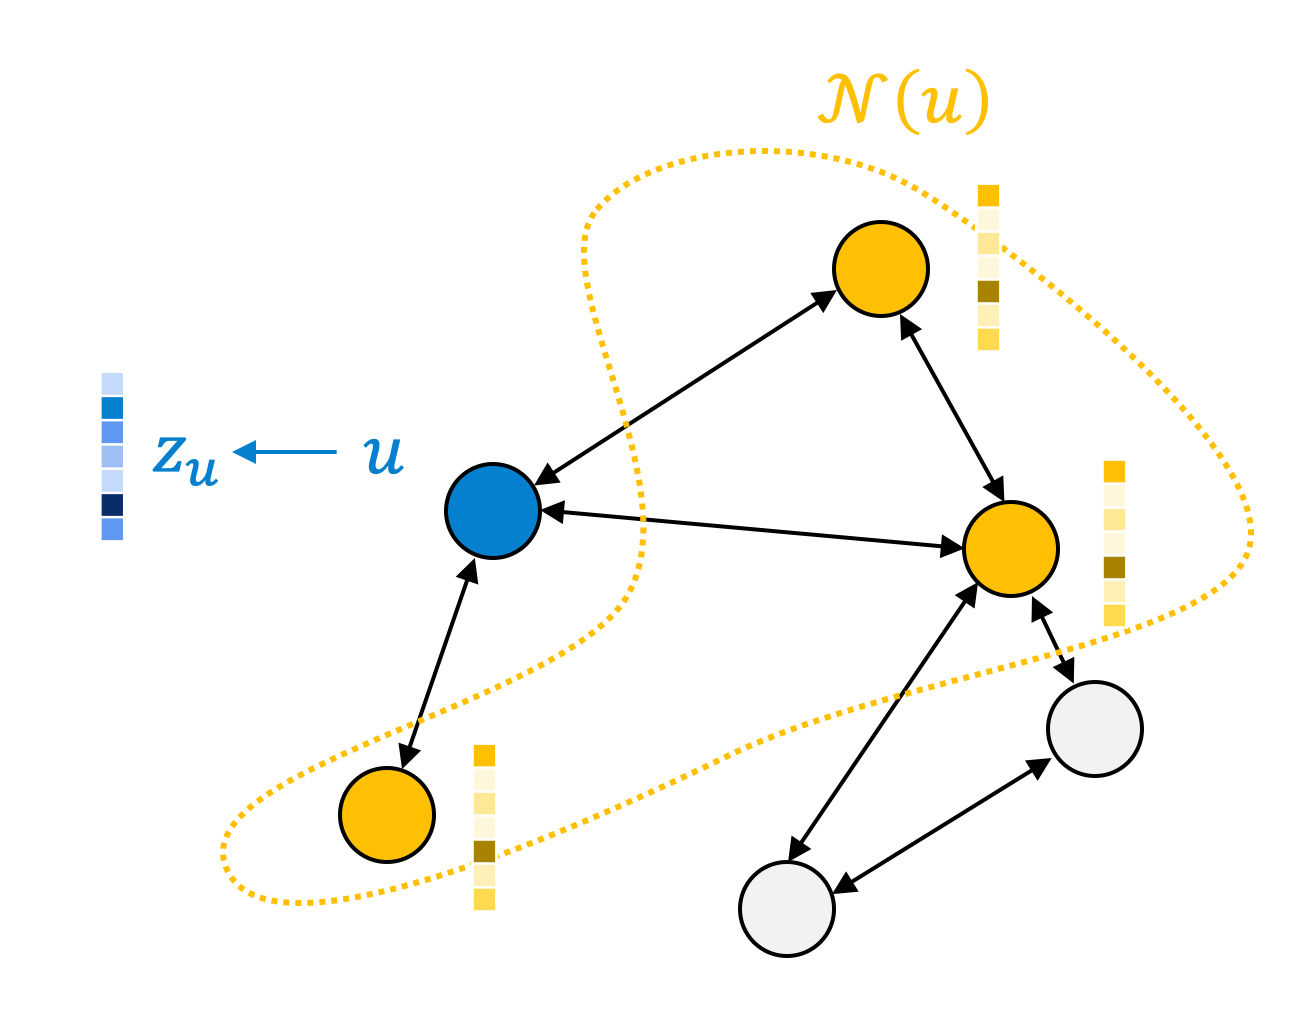
\includegraphics[width=8cm]{images/graph-neihborhood_2.png}
\end{center}
\caption{Illustration of a graph neural network (GNN) applied to an instance of a graph. The graph neural network takes the graph along with a set of node features (represented as vectors on the figure) as input and associates each node $u \in \mathcal{V}$ from the graph to an embedding $z_u$. For the node $u$ (in blue), we illustrate its neighborhood $\mathcal{N}(u)$  as all the nodes directly connected to $u$ (in yellow).}
\labfig{graph-example}
\end{figure}

Graph neural networks take as input a graph $\mathscr{G}$ along with a set of node features $X \in \mathbb{R}^{d \times |\mathcal{V}|}$, with $d$ the network hidden size. We illustrate a graph neural network in \reffig{graph-example}.
Graph neural networks generate a node embedding $z_u, \forall u \in \mathcal{V}$. They iteratively update node hidden embeddings $h_u^{(k)}$ using a neural message passing process. 
We can decompose each iteration in two steps: First, an \textit{aggregation} step (\refeq{aggregate}), that aggregate the information from all nodes directly connected to $u$, that we define as the graph neighborhood $\mathcal{N}(u)$. Then an \textit{update} step (\refeq{update}) that update each hidden embedding given its neighborhood aggregated information and its previous state. We illustrate the iterative process in \reffig{gnn}. 

\begin{align}
    m^{(k)}_{\mathcal{N}(u)} &= \mathsf{aggregate}^{(k)}\left(\{h_v^{(k)}, \forall v \in \mathcal{N}(u)\}\right), \labeq{aggregate} \\
    h^{(k+1)}_u &= \mathsf{update}^{(k)}\left(h^{(k)}_u, m^{(k)}_{\mathcal{N}(u)}\right), \labeq{update}
\end{align}

Here, the $\mathsf{aggregate}$\sidenote{The $\mathsf{aggregate}$ function takes a set as input and is therefore permutation invariant by design.} and $\mathsf{update}$ function are differentiable and $m_{\mathcal{N}(u)}$ is the \textit{message} aggregated from $u$ neighborhood. 

\begin{figure*}[!htb]
\begin{center}
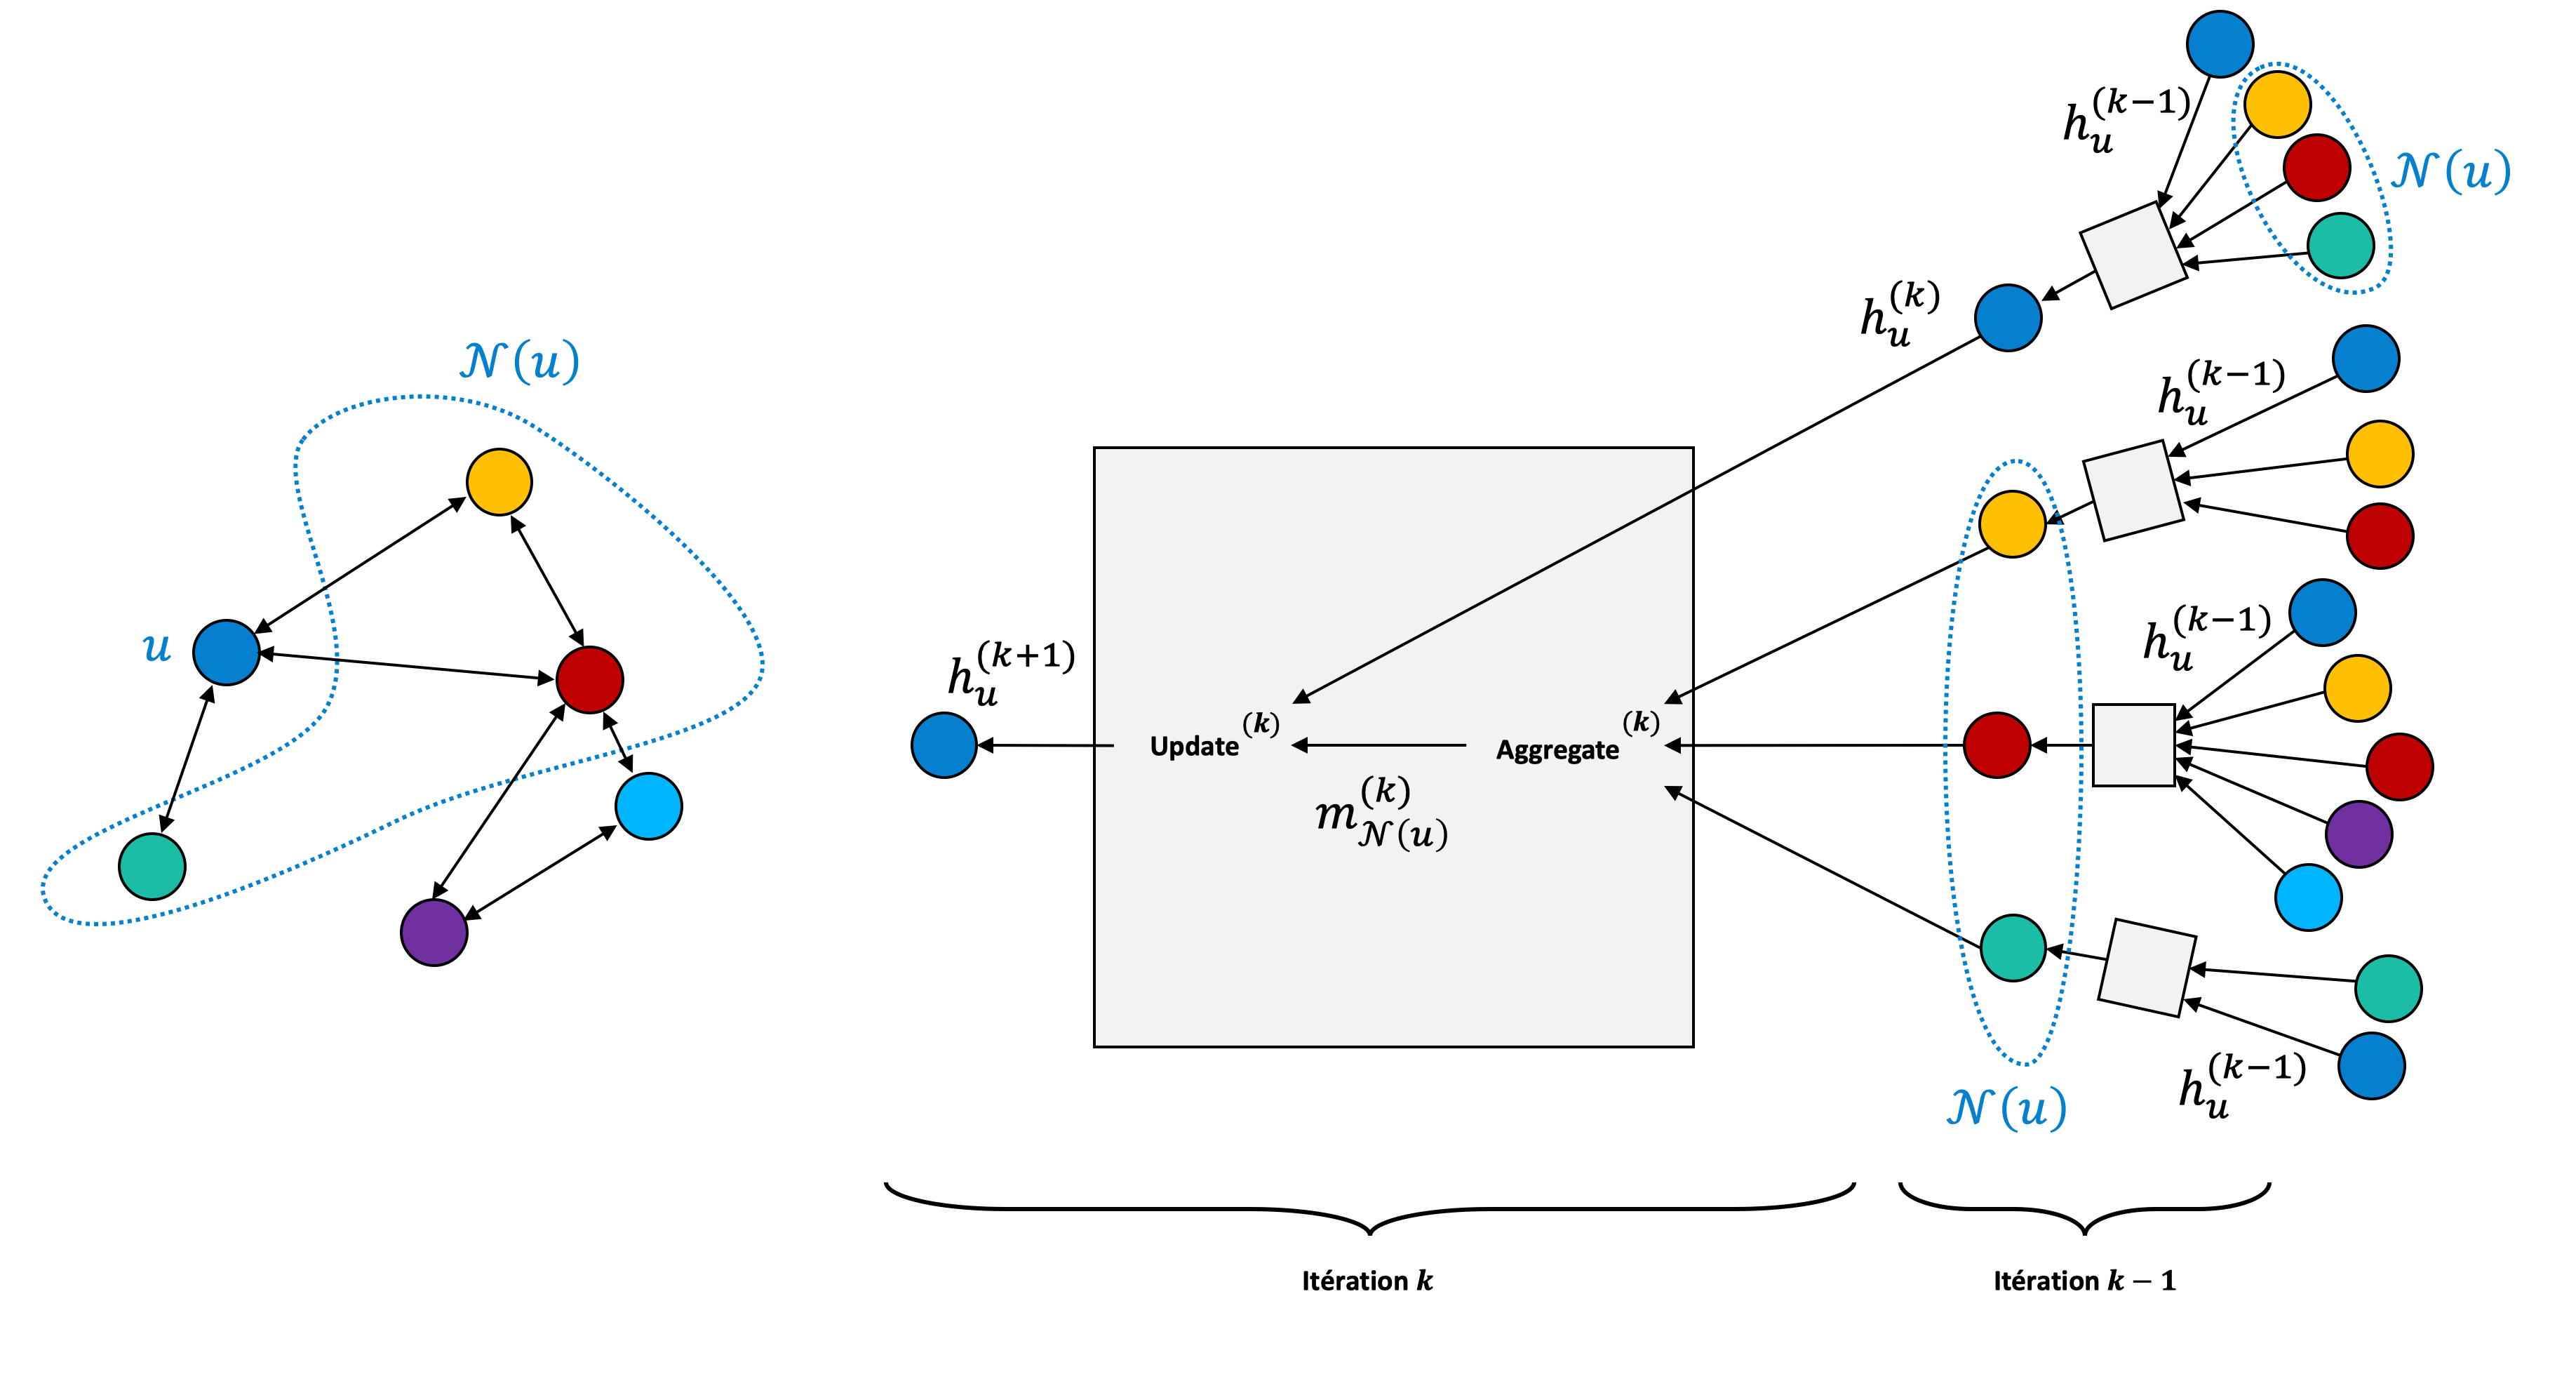
\includegraphics[width=16cm]{images/graph_update_5.png}
\end{center}
\caption{Illustration of one iteration to compute the hidden state of the node $u$ (in dark blue). We decompose the iteration in two steps: the aggregation (\refeq{aggregate}) and update (\refeq{update}) step. We illustrate two iterations, at step $k$ to compute $h_u^{k+1}$ and $k-1$ to compute $h_u^{k}$. We adapted the figure from \textcite{hamilton_2020}.}
\labfig{gnn}
\end{figure*}

For simplification, we can add self-loops to the input graph such that $u$ is included in its own neighborhood $\mathcal{N}(u)$. 
The message passing iteration can then be defined using a single equation and we implicitly define the \textit{update} step in the \textit{aggregate} step (\refeq{update-aggregate}). We illustrate the iterative process with this simplification in \reffig{gnn-2}. 

\begin{equation}
    h^{(k+1)}_u = \mathsf{aggregate}^{(k)}\left(\{h_v^{(k)}, \forall v \in \mathcal{N}(u) \cup \{u\}\}\right), \labeq{update-aggregate}\\
\end{equation}

\refeq{embeddings} defines the embedding of each node as its hidden state after $K$ message passing iterations:

\begin{equation}
    z_u = h_u^{(K)}, \forall u \in \mathcal{V}, \labeq{embeddings}\\
\end{equation}

At each iteration, each node aggregates information from its $k$-hop neighbors. Node embeddings, therefore, encode structural and feature-based information.

\begin{figure*}[!htb]
\begin{center}
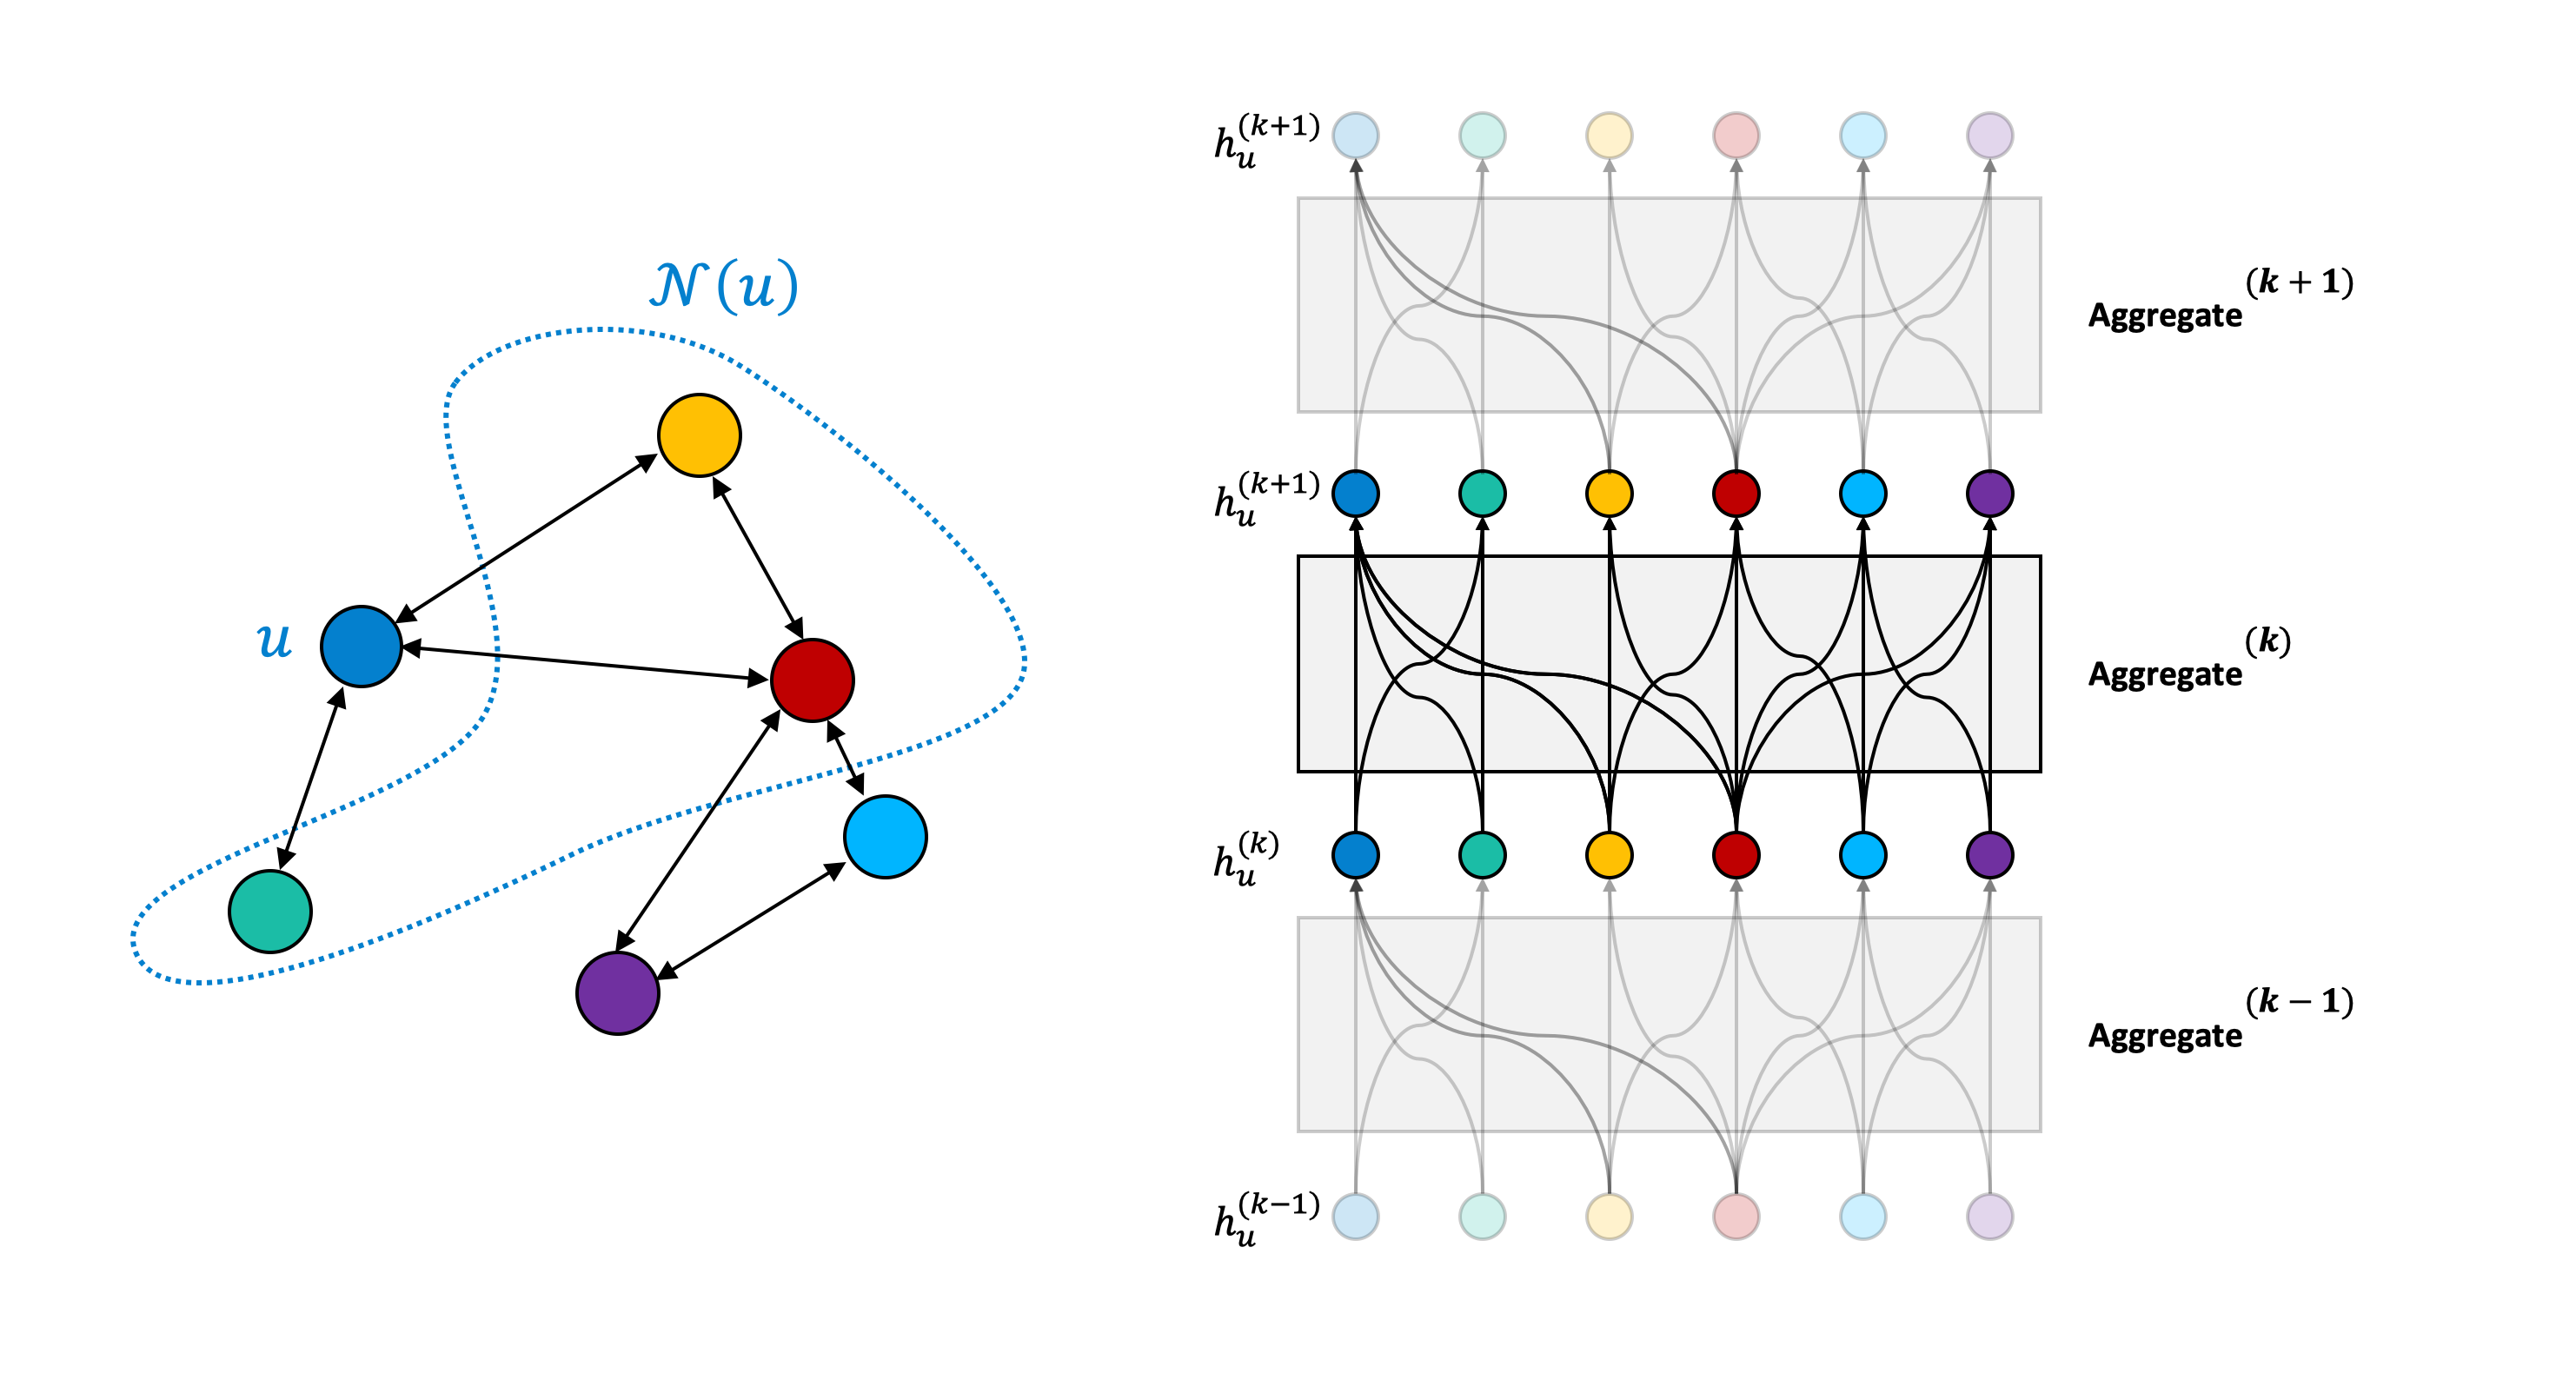
\includegraphics[width=16cm]{images/graph_update_7.png}
\end{center}
\caption{Illustration of one iteration to compute the nodes hidden state. We include each nodes in its own neighborhood $\mathcal{N}(u)$ and thus implicitly define the \textit{update} step in the \textit{aggregate} step (\refeq{update-aggregate}). We illustrate iterations, at step $k$ to $k+1$.}
\labfig{gnn-2}
\end{figure*}

\subsection{Defining transformer's message passing functions}

Transformers \parencite{vaswani_17} may easily be defined under the graph neural network framework. 
They transform inputs through a fixed number of layers.
As detailed in \refsec{architectures:transformers}, each layer is composed of a multi-head attention (MHA) block and a feed-forward network (FFN).
The self-attention mechanism that transforms a \textit{set of vectors} into what is known as \textit{contextualized vectors}. 
Each contextualized vector is a weighted average of the vectors from the original set.
% They operate on a set of vectors. 
Since attention composes every vector from the set, we can consider that transformers operate on fully connected graphs.
We can adapt the \refeq{update-aggregate} for transformers and compute the contextualized representation $h_u$ of given token $u$ in an input text as follow\sidenote{In fact, we can also formally decompose transformers layers by considering the MHA layer as the $\mathsf{aggregate}$ function and the FFN layer as the $\mathsf{update}$ function. This interpretation may provide a formal background to analyze the role of the FFN.}:

{\small
\begin{align}
    h^0_u &= W^{(e)} u + W^{(p)} \labeq{update-aggregate-transformers-emb}\\
    h^{(k+1)}_u &= \text{FFN}^{(k)}\left(\text{MHA}^{(k)}\left(\{h_v^{(k)}, \forall v \in \mathcal{N}(u) \right) + h_v^{(k)}\right), \labeq{update-aggregate-transformers}
\end{align}}
% \cup \{u\}\}

Where \refeq{update-aggregate-transformers} is the first layer that encodes words using $W^{(e)}$ embedding layer summed with positional embeddings layer $W^{(p)}$. The neighborhood $\mathcal{N}(u)$ of each token $u$, corresponds to every token in the sentence, including the token $u$ itself.

\subsection{Tricks and limits}

We can interpret transformers as GNNs operating on a fully connected graph. However, in the specific case of NLP, transformers should preserve the information about the sequential order of words. In that regard, transformers borrow common tricks and mechanisms from graph neural networks.

The transformer formalization encodes the linear order of words in the positional embedding layer $W^{(p)}$ from  \refeq{update-aggregate-transformers-emb}. We can interpret the un-contextualized embeddings $h^0_u, \forall u \in \mathcal{V}$  as the set of initial node features $X \in \mathbb{R}^{d \times |\mathcal{V}|}$ defined in \refsec{gnn:definitions}. As a result, the message passing iteration defined in \refeq{update-aggregate-transformers} is permutation invariant, a standard property in traditional graph neural networks.
%  used to generate node contextualized embeddings $z_u, \forall u \in |\mathcal{V}|}$

It is also essential to preserve the word information across the iterations such that $h^{(k)}_u$ indeed captures the contextualized information about the token $u$. This issue of preserving token identities is addressed using the skip connection: before and after the FFN layers, we add the source to the current hidden state. The same mechanism is also commonly used in GNNs to avoid over-smoothing. As detailed in \textcite{hamilton_2020}, this issue happens when node-specific information is lost after several message passing iterations. In such a case, the representation of every node tends to become very similar. Commonly this issue is addressed by including the previous hidden state together with the aggregated state in the computation of the updated state.
This skip connection aims at explicitly preserving information from the previous iteration during the update.
% As detailed in \refsec{gnn:definitions}, GNNs take as input a graph $\mathscr{G}$ along with a set of node features $X \in \mathbb{R}^{d \times |\mathcal{V}|}$, to generate node embeddings $z_u, \forall u \in \mathcal{V}$. In our interpretation, node features correspond to embeddings $h^0_u, \forall u \in \mathcal{V}$ obtained with \refeq{update-aggregate-transformers-emb}. 

% \bcomment{???}{}This approach depends on the arbitrary ordering of nodes that we used in the adjacency matrix.


% \bcomment{preserve word identities in NLP ?}{}

% Another common pitfall of graph neural networks \bcomment{is that every nodes may have a different degree}{is that nodes have different degrees}.  This may affect the scale of the vector during aggregation. This variance in scale may results in numerical and optimization instability. \bcomment{does it apply to transformers in NLP ?} A common way to alleviate this issue is to normalize the operation based upon the degree of nodes involved. The normalization is also a sensitive operations of transformers (see csordas) \bcomment{???}{sth missing here}



\subsection{Interpretation}

The formalization of transformers as graph neural networks opens an original angle to interpret them.
The mechanism of transformer layers is often compared to intuitive NLP pipelines \parencite{tenney_19}. 
Starting with the lower layers encoding surface information, middle layers encoding syntax, and higher layers encoding semantics \parencite{jawahar_19, peters_18}.

In the graph neural network perspective, we conjecture that transformers progressively refine the feature through an iterative message passing process.
As described in \textcite{xin_20}.  become more fine-grained at each iteration.
This also provide a new interpretation path for \textsc{Albert} \parencite{lan_20}.
The model is based on the transformer architecture, except that weights are tied across layers.
In out GNN interpretation, the model uses the same message passing function at each iteration such that, in \refeq{update-aggregate-transformers}, the functions $FFN^{(k)}$ and $MHA^{(k)}$ are the same for each iteration $k$.

\subsection{Graphs, trees, sequences}
\labsec{transformers:graph}

It is also possible to extend the graph neural network formalism for other NLP models.
Tree-structured models operate on trees, which are directed acyclic graphs.
The Tree-LSTM equations are detailed in \refsec{architectures:tree}.
They may also be formatted in  $\text{aggregate}$ and $\text{update}$ functions.
In this case, the $\text{aggregate}$ function consists of the simple sum of the node neighborhood hidden states.
A key aspect is that the graph defined by Tree-LSTM does not contain any loop.
the message passes in a bottom-up manner, starting from the leaf to the root. Since they have no dependant, the leaf nodes computation will be the same after the first iteration such that $\forall k \ge 2, h_u^{(k)} = h_u^{(k+1)}$. Similarly, for the computation of the leaf node parents, the inputs will be the same starting from the second iteration. After a number of iterations equal to the tree-depth, the value of all node hidden states will be determined.
% In this case, there is only a single message passing iteration. \bcomment{why ? you might actually iterate ?}{even if probably useless}


\begin{figure}[htb!]
    \centering
    \begin{subfigure}[b]{0.475\textwidth}
        \centering
        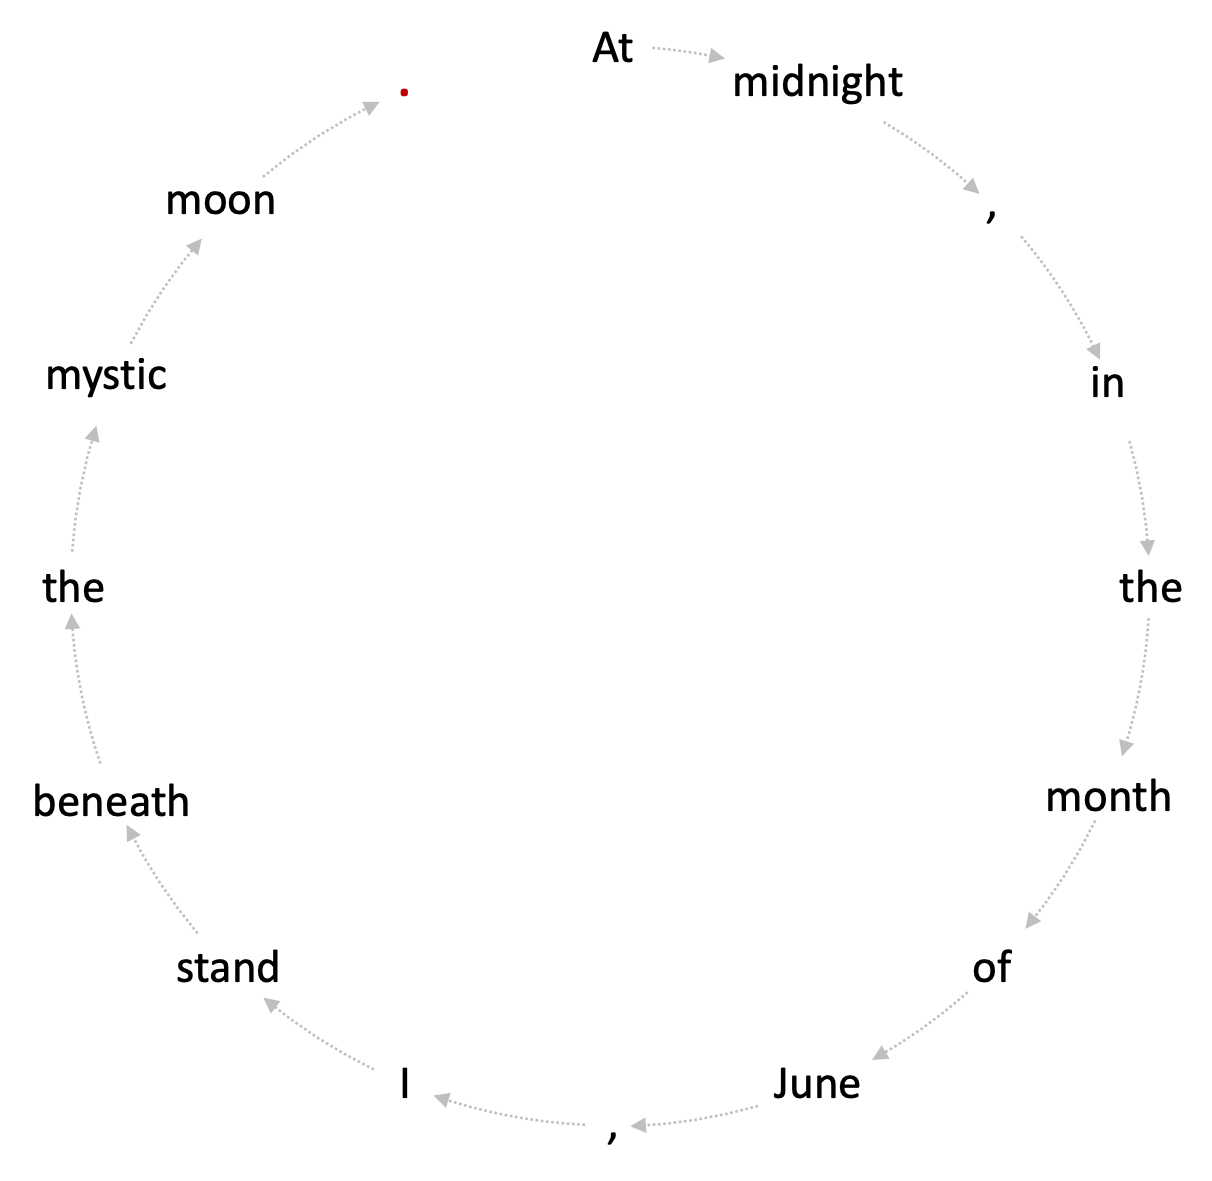
\includegraphics[width=\columnwidth]{images/rnn_uni.png}
        \caption{Unidirectional RNN}
        \labfig{subfig:structure-1}
    \end{subfigure}
    \hfill
    \begin{subfigure}[b]{0.475\textwidth}  
        \centering 
        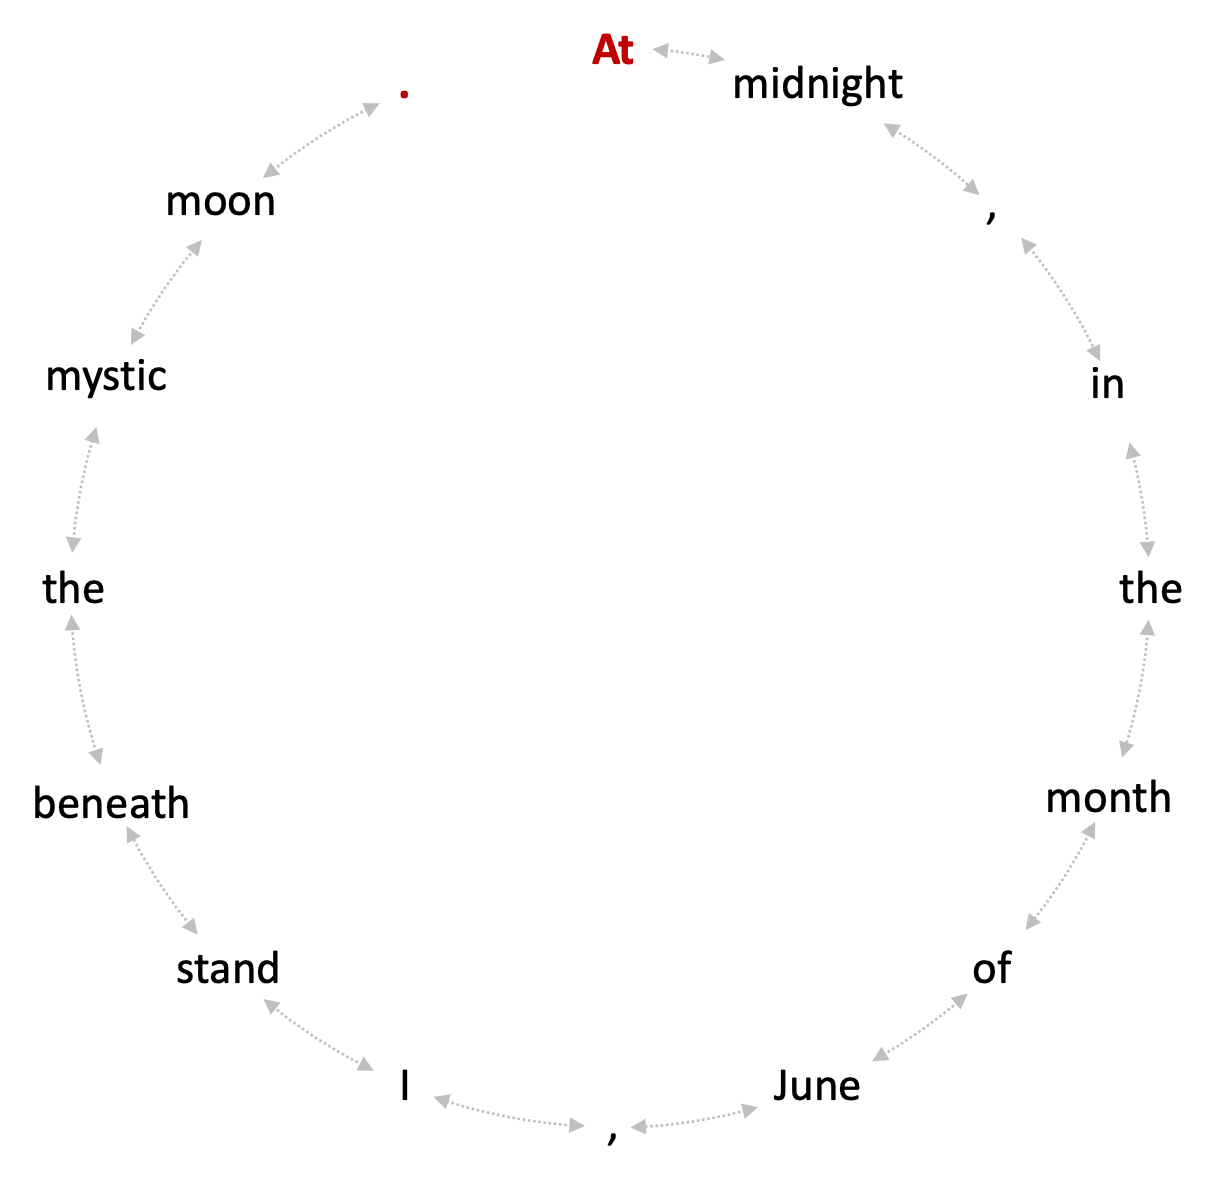
\includegraphics[width=\columnwidth]{images/rnn_bi.png}
        \caption{Bidirectional RNN}
        \labfig{subfig:structure-2}
    \end{subfigure}
    \vskip\baselineskip
    \begin{subfigure}[b]{0.475\textwidth}   
        \centering 
        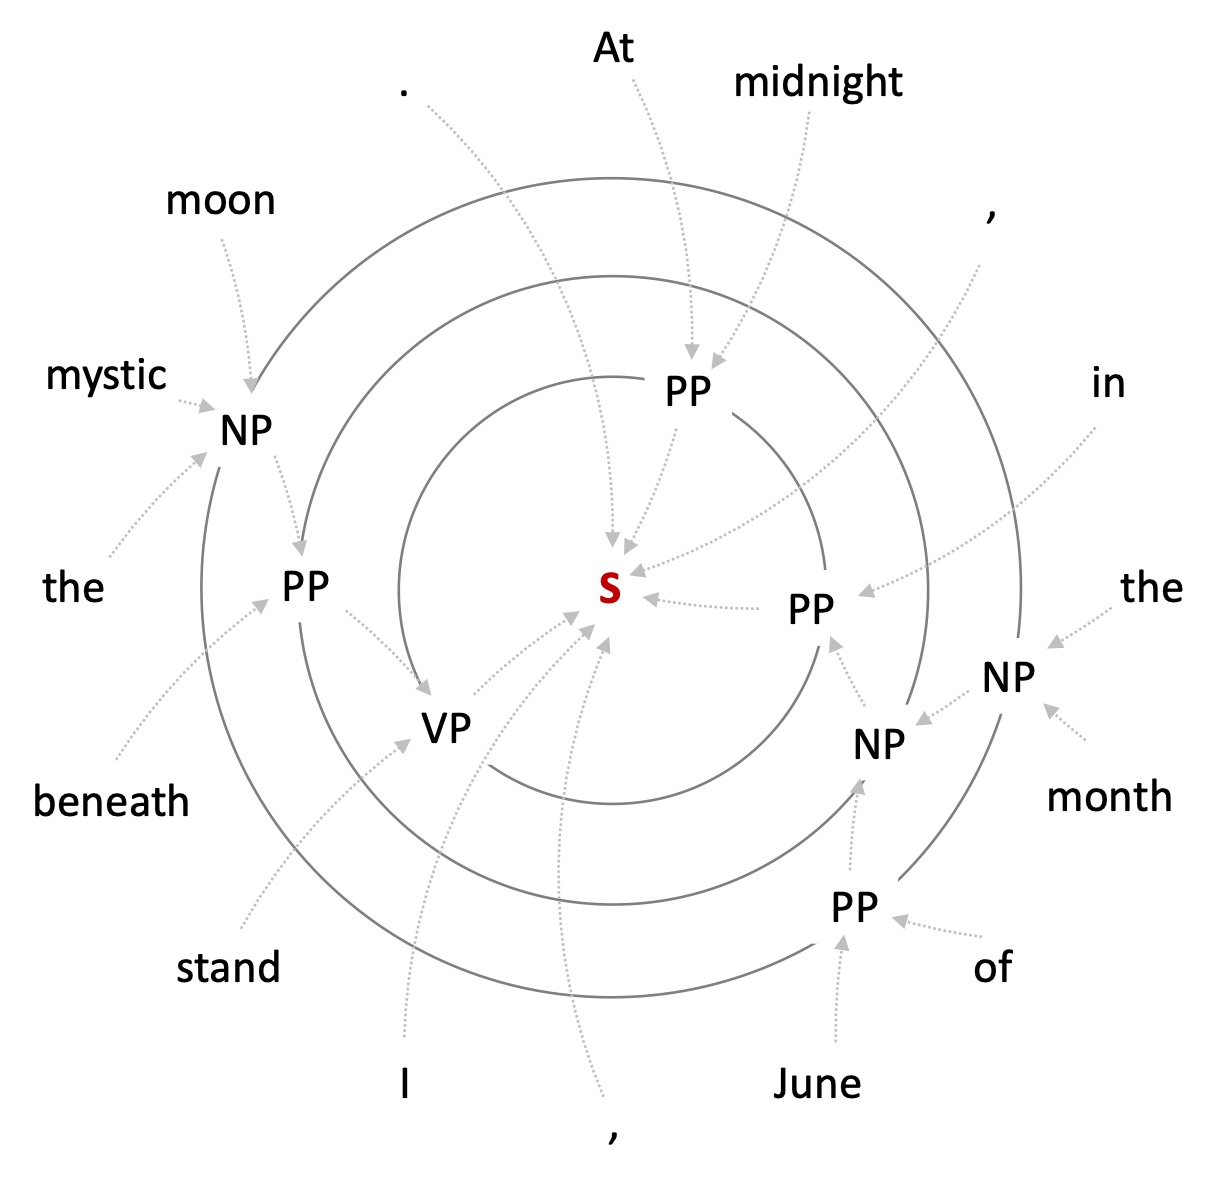
\includegraphics[width=\columnwidth]{images/rnn_const.png}
        \caption{N-ary Tree RNN}
        \labfig{subfig:structure-3}
    \end{subfigure}
    \hfill
    \begin{subfigure}[b]{0.475\textwidth}
        \centering 
        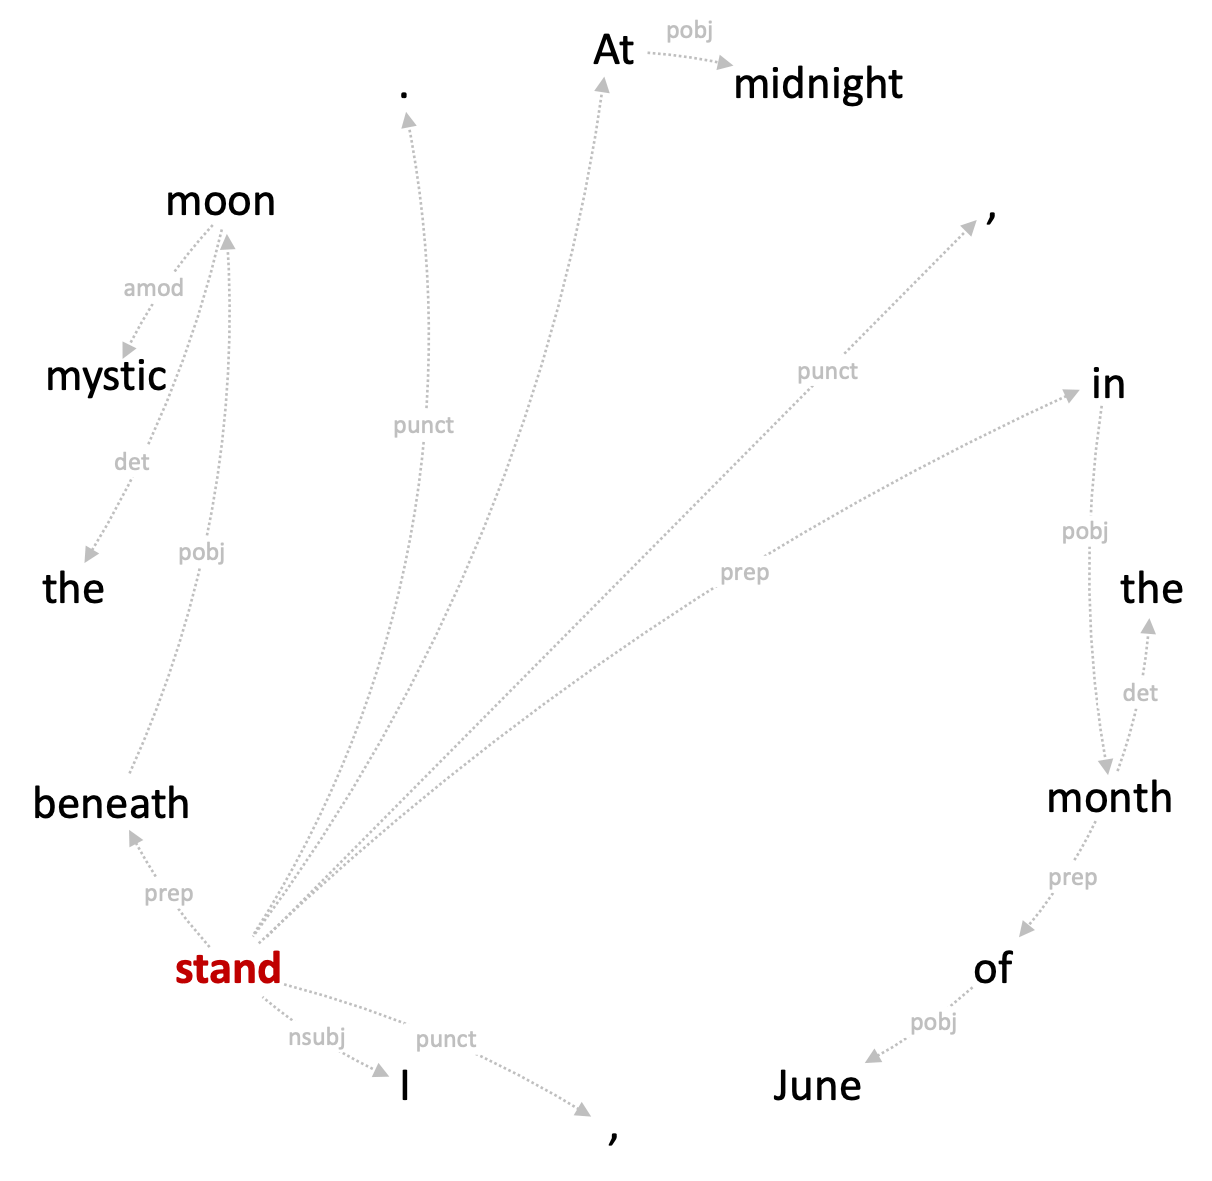
\includegraphics[width=\columnwidth]{images/rnn_dep.png}
        \caption{Childsum Tree RNN}
        \labfig{subfig:structure-4}
    \end{subfigure}
    \vskip\baselineskip
    % \begin{subfigure}[b]{0.475\textwidth}
    %     \centering
    %     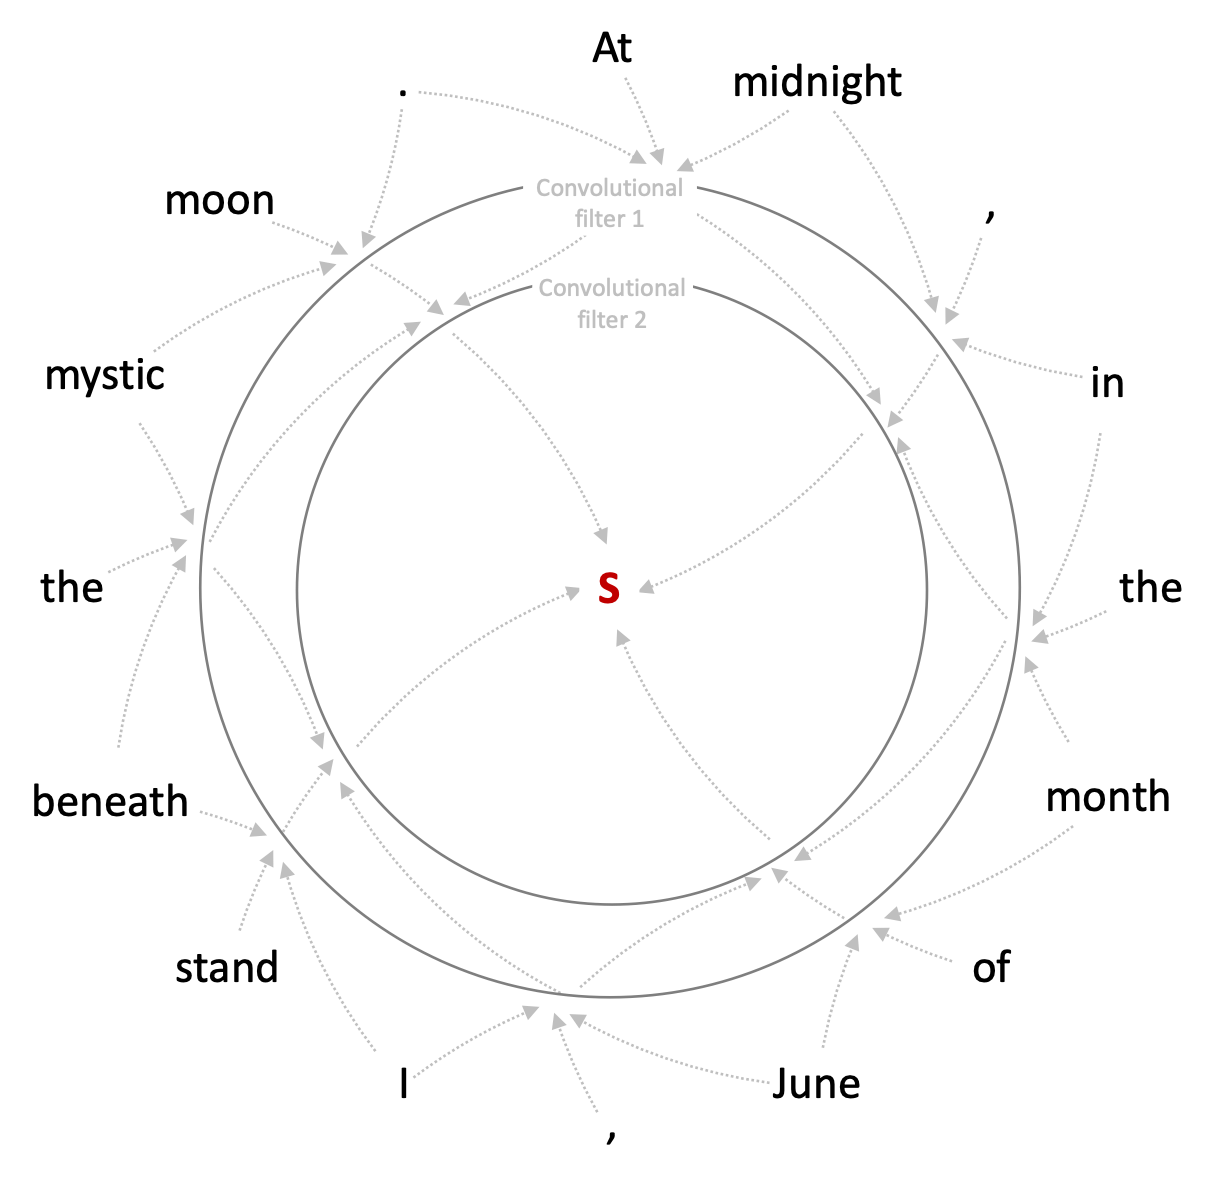
\includegraphics[width=\columnwidth]{images/conv.png}
    %     \caption{Convolutional NN}
    %     \labfig{subfig:structure-5}
    % \end{subfigure}
    % \hfill
    \raggedright
    \begin{subfigure}[b]{0.475\textwidth}  
        \centering 
        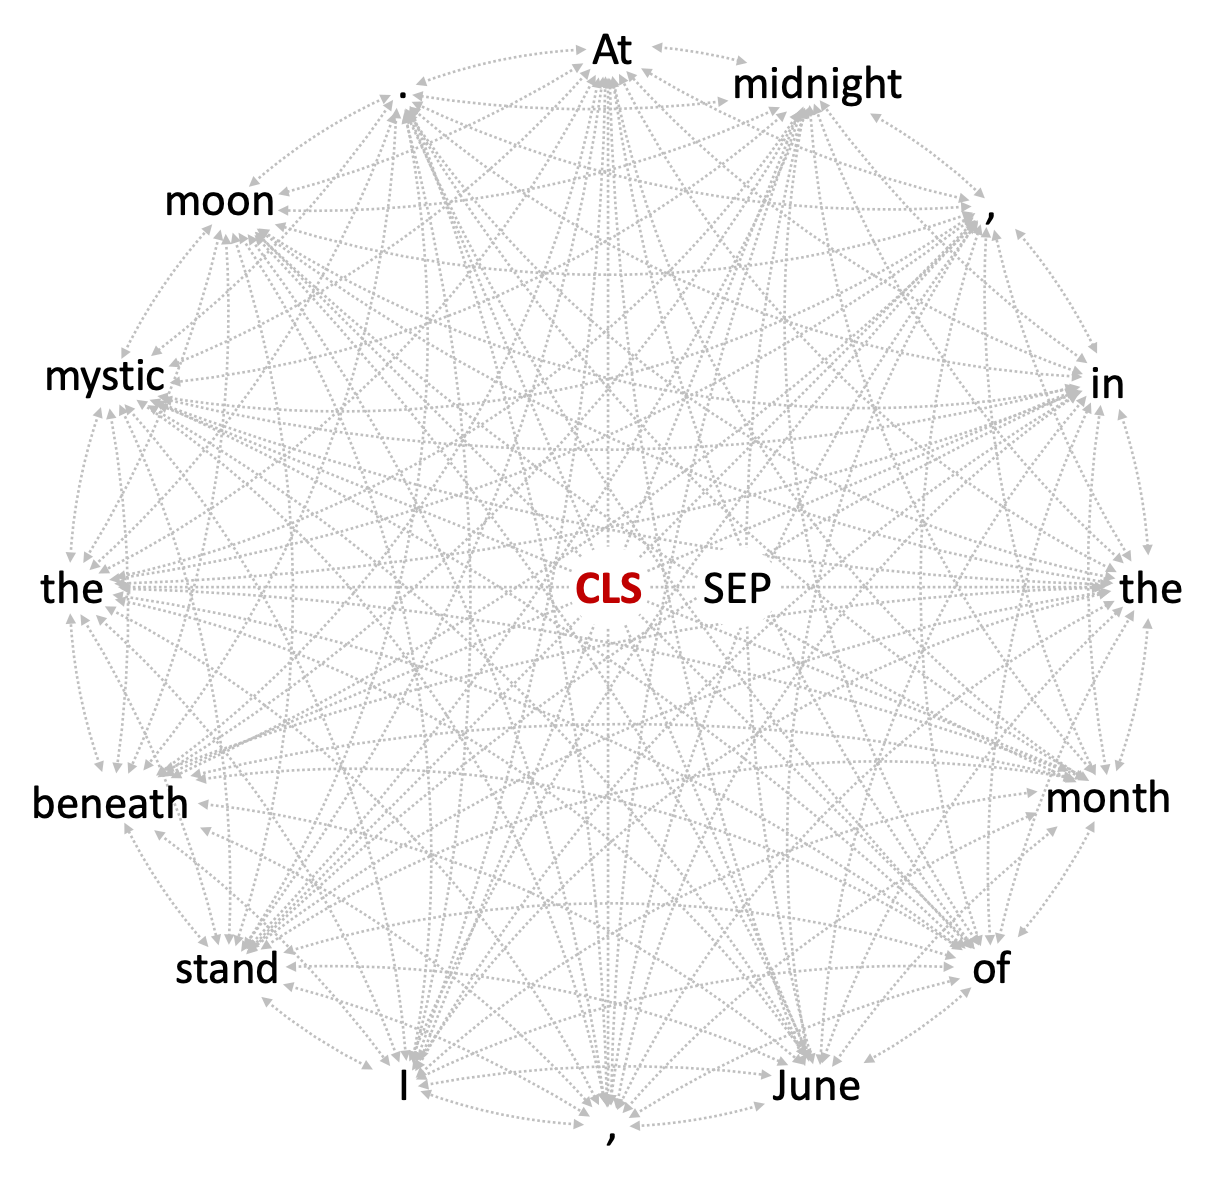
\includegraphics[width=\columnwidth]{images/transformer.png}
        \caption{Transformer NN}
        \label{subfig:structure-6}
    \end{subfigure}
    \hfill
    \caption{Latent structure for distinct standard NLP architectures. Illustration on the first line of the poem: "The Sleeper" by Edgar Allan Poe (published 1831). We obtain the constituency tree for \reffig{subfig:structure-3} using Berkley neural parser \parencite{klein_18}. For \reffig{subfig:structure-4}, we parse the sentence using the dependency parser from Spacy (\url{https://spacy.io/api/dependencyparser}) \parencite{honnibal_15}.} 
    \labfig{structure}
\end{figure}

Sequential LSTM may also be considered a particular kind of graph neural network. 
A sequence is indeed equivalent to an unary directed acyclic graph.
As for the \textsc{Tree-LSTM}, the \textsc{LSTM} equations may also be separated in a $\text{aggregate}$ and $\text{update}$ functions.
In this case, the $\text{aggregate}$ function is just the identity function since each node has exactly one child.
As for the \textsc{Tree-LSTM}, after a number of iterations equal to the sequence length, the value of all node hidden states will be determined.

We illustrate the input structure corresponding to the different architectures in \reffig{structure}.
Sequential \textsc{RNN} or \textsc{TreeRNN} operate on sparse graph structure. Node and edge numbers are equivalent in order of magnitude: $|\mathcal{V}| \approx |\mathcal{E}|$. On the contrary, transformer operate on a fully connected graph. The number of edges equals number of nodes squared: $|\mathcal{E}| = |\mathcal{V}|^2$.

\subsection{Are transformers over-parametrized?}

% Il faut parler du pruning qui justifie que graph dense pas forcement nécessaire !! Sauf pour ettinger et distill bert

It looks like the answer is included in the question. 
Transformers are indeed admittedly over-parametrized in the litterature \parencite{chen_20, hou_20, voita_19}. 
Yet, the role of this over-parametrization is not well understood. 
Transformers layers are suspected to be highly redundant \parencite{liu_20} and to cause over-fitting \parencite{fan_20, zhou_20b}. 

In the light of our GNN analysis transformers should naturally share parameters across layers. As mentioned earlier, the model \textsc{Albert} \parencite{lan_20} already implements this key specificity by tying weights across layers. Similarly, \textsc{Tree-LSTM} or sequential \textsc{LSTM}, which can be interpreted as GNN other specific graphs, also share their parameters across iterations.

However, the critical distinction between transformers and trees and sequences recurrent neural networks is the properties of the latent graph structure. Tree and sequences will converge after a finite number of message passing iterations since they do not include any loop within their structure. However, transformers operate on a fully connected graph. Token hidden states cannot be computed in a given hierarchical order since they all depend on each other.

We hypothesize that token hidden states will eventually converge toward a fixed point\sidenote{In that matter, \textcite{zhou_20c} states that such fixed point is uniquely defined with the assumption that $\mathsf{aggregate}$ is a contraction map in \refeq{update-aggregate}. By definition a contraction map is a function such that there is some non negative real number $0\leq k<1$ such that for all vector $x$ and $y$, $d(f(x),f(y))\leq k\,d(x,y)$, with $d$ a distance metric over our vector space.} We also hypothesize that some tokens require more iterations than others and that this convergence process will depend on the word and its context. Indeed, many studies show that the weighted graph formed by attention weights is not homogeneous. Some tokens contribute in large proportion to the update of the other, while some have a marginal or null contribution to the attention weights.

% As observed in \labsec{sec:parses-impact}, these tree might have little in common

% In this Section, we aim at better defining and characterizing the notion of structure for data and computations\sidenote{\textcite{battaglia_2018} argue that "combinatorial generalization must be a top priority for AI to achieve human-like abilities, and that structured representations and computations are key to realizing this objective.".}.

% \subsection{Structured neural networks} 

% \bcomment{this section is messy}{what is your point, the computation graph is not the key abstraction, that's the message passing (see below)}

% Artificial neural networks consist of connected units called neurons. Neurons define a vector space transformation based on linear algebra operators and nonlinear activation functions. Neural networks typically contain a very large number of neurons, which may be arranged into layers. Neurons—and by extension layers—are inter-connected: they receive input from their inner connections and send their output to their outer connections. Each layer has its own inner structure and connection pattern. The collection of layers and their connections forms a directed \textit{computational graph}. 
% Feed forward networks produce a directed acyclic computational graph. But Recurrent networks allow for connection between the same or previous layer, thus introducing cycles in the computational graph.

% Static neural networks have a fixed computational graph. In such case, inputs are all formatted according to a given standard, for instance images with $64 \times 64$ pixels. While the inputs numerically differ, they all follow the same sequence of transformation across layers. Other networks (such as the \textsc{LSTM} and \textsc{TreeLSTM} introduced in \refch{tree}) process inputs with variable format. In this case, the computational graph varies for each input sample\sidenote{We refer to such architectures as dynamic networks \parencite{han_2021}.}. Sequential recurrent networks operate with sequences as input, tree recurrent networks with trees. Sequences and trees induce a notion of hierarchy. We can assign: an index to each element in a sequence, based on their order~; a depth to each element in a tree, based on the length of the shortest path to the root node. This hierarchy directly impacts the computational order of the corresponding architectures. For recurrent or recursive neural networks, the computational graph follows the topological structure of the input, respectively a sequence or a tree.

% Sequential recurrent networks process words sequentially given their order. Tree recurrent networks process words in a bottom up manner: starting from the leaves, up to the root.
% Transformers operate on fixed length input and apparently \bcomment{fall on the static network category}{nope, the computation graph is different for sentences with different lengths (in theory), same computation is practical}. As \textcite{hamilton_2020, joshi_2020}, we argue in the next section that we may interpret transformers as a structured network operating on fully connected directional graph.
% We refer to intermediate layer outputs as hidden states. 

% Neural networks process samples trough the layers, along with the computational graph. We refer to intermediate layer outputs as hidden states. The hidden states consist of latent distributed representations. They are not design such that their coordinates reflect some specific semantic information. Yet, for the architectures introduced in \refsec{training:architectures} (\textsc{LSTM}, \textsc{TreeLSTM}, or transformers) it is possible to associate the hidden states $h_t$ to a specific word $w_t$ from the input sequence.

% We refer to the graph defined by the collection of layers and their connections as the network structure. If the network structure is a directed acyclic graph, we refer to the model as a feed forward network. If the network structure allow connection between the same or previous layer, we called it a recurrent network. Finally, recursive neural networks allow connection if the form of a given tree topological order. 

% Interestingly, the network structure may be defined regarding the input structure...

% Artificial neural networks are a collection of connected units called neurons. Neurons are connected to each others in various patterns. The network of the neurons and their inner connection forms a directed, weighted graph.

% Since their introduction, deep learning models have strongly evolve. While, in theory, they could express any function using a sole MLP layer. In practise, Their architectures evolve and overcome their practical constraints. Such as gradient overflow. In recent architectures, we introduce inductive biases. and not dense connection. We can interperet these choosen connections using graphical models.

% Structure is not a well define notion.
% It can points to the inherent structure of the input. For examples, molecules have a structure describe by their atoms and the link between them. 

% This structure can be more fuzzy. Some atoms links are differents and less trong than others. Language is often describe using a recursive tree structure and several formalism exists. Images may also be describe by meta elements and the link between them.

% This structure is also different from the model structure use to encode the elemnts. For example, molecule can be encoded using a sequential recurrent networks, relying on a sequential structure. But some mechanisms may help to account for the recursive structure such as memomry cell (c.f. eaxmples verbs subject agreement)

% In this section we aim at precisely defining the notion of structure.

% We define the input of the input as a set of elements $W$ and a set of relations between them $S$.

% We define the structure of the model as the element and the computational order in which their are computed. (pas exactement ça putot définition enf contion des entrée sorties).

% \subsection{Graph Structure} 

% \bcomment{potential structure for the whole beginning of chapter}{
% Providing a clear view on transformers would be real plus value of this chapter (insightful for many readers). It is worthwhile to spend time on it. Start with Graph neural networks (abstract graph based presentation, see Hamilton):
% \begin{enumerate}
% \item State that you analyze transformers as a GNN with message passing between the node embeddings of the GRAPH (Hamilton). And provide a schema or two like Hamilton\\
% \item It entails that transformers are iterative, it explains there are many layers
% \item State that the heads and the feedforward connections are part of the extra stuff + the parametrization of each layer + positional embeddings 
% \item Once it is done. Explain that in the case of language and with transformers the graph considered is fully connected.
% \item Then and only then, explain that you can compare the message passing behavior of transformers to the message passing behavior of the other models (your plots in Fig 5.1 are insightful bc they show the extra connectivity of transformers.
% \item You might also stress that transformers do iterative refinements while other models (LSTMSs) do not. Yet, how does the message passing looks like with stacked LSTMs ?
% \end{enumerate}
% To summarize, do not mess up with the computation graph, but rather take advantage of the message passing framework of Hamilton
% }


% \bcomment{I disagree with some of your plots}{for the LSTM plots, I would add (or at least mention) indirect arcs that connect each word to ALL its predecessors, same for tree LSTMs}

% % Many data exhibit an explicit structure. 
% We define a graph $\mathscr{G}$ by a tuple of sets $\mathscr{G} = (\mathcal{V}, \mathcal{E})$. With $\mathcal{V}$ the set of vertices and $\mathcal{E}$ the set of edges between the node. A graph is a ubiquitous data structure that can describe many complex systems. For example, molecules are a group of atoms held together by chemical bonds. Chemical graphs are full-fledged representations of them, with vertices corresponding to atoms and edges to chemical bonds.

% \begin{table}[!htb]
%   \small
%   \centering {
%   \begin{tabularx}{\textwidth}{YYYc}
%     \toprule
%     \textbf{Architecture} & \textbf{Data structure} & $\mathcal{V}$ & $\mathcal{E}$\\
%     \midrule
%     \textsc{LSTM} & Sequence & $\{w_i\}_{i \in \llbracket 1, N \rrbracket}$ & $\{(w_i, w_{i+1})\}_{i \in \llbracket 1, N \rrbracket}$\\
%     Childsum \textsc{TreeLSTM} & Tree & $\{w_i\}_{i \in \llbracket 1, N \rrbracket}$ & $\{(w_i, w_{j})\}_{i \in \llbracket 1, N \rrbracket, j \in C(i)}$\\
%     Nary \textsc{TreeLSTM} & Tree & $\{w_i\}_{i \in \llbracket 1, N \rrbracket} + \{c_i\}_{i \in \llbracket 1, M \rrbracket}$ &  $\{(w_i, w_{j})\}_{i \in \llbracket 1, N \rrbracket, j \in C(i)}$\\
%     Transformer & Graph & $\{sw_i\}_{i \in \llbracket 1, N \rrbracket}$ & $\{(sw_i, sw_{j})\}_{i, j \in \llbracket 1, N \rrbracket}$ \\
%     \bottomrule
%   \end{tabularx}}
%   \caption{For each sentence encoder architecture, we pair a sentence data structure. We formalize each structure as a specific graph. We describe sequences as unary directed acyclic graph and tree as directed acyclic graph. We associate transformers to fully connected directed graph as argued in \refsec{transformers:structure}. We notations defined in \refsec{training:architectures}: $w$ corresponds to a word and $sw$ to a subwords. $c$ are consitutents. $C(j)$ denote the set of children of node $j$.}
%   \labtab{graph-structure}
% \end{table}

% Regarding language, we can decompose a sentence using the linear order of words. In this case, we represent the sentence by an \textit{ordered sequence} of words $W = (w_1, w_2, \cdots, w_N)$. An equivalent formalism will be to represent the sentence as a \textit{set} of words $\mathcal{V} = \{w_1, w_2, \cdots, w_N\}$ and a set of relations between them $\mathcal{E} =\{(w_i, w_{i+1})\}_{i=1 \cdots N}$. In \reftab{graph-structure}, we formalize the input structure of \textsc{LSTM}, Childsum \textsc{TreeLSTM} and Nary \textsc{TreeLSTM} as graphs.

% % Dependency parsing describe the sentence as a tree for which each node corresponds to a sentence word and each vertex corresponds to a relation between two words. Formally, the sentence can still be described as as a \textit{set} of words $W$ and a set of relations between them $S$. However, in such case, the set of relations will describe a tree. Finally, constituency parsing describes the sentence as a tree. Except, intermediary nodes are used. We can still use the same formalism but we need to include intermediate consituents in the definition: a \textit{set} of words and constituents $W = \{w_1, w_2, \cdots, w_N, c_1, c_2, \cdots, c_M\}$.

% \subsection{Transformers as graph neural networks}
% \labsec{transformers:structure}

% % Transformers introduce a deep paradigm shift in NLP neural architectures. 
% Transformers rely on self-attention: a mechanism that transforms a \textit{set of vectors} into what is known as \textit{contextualized vectors}. Each contextualized vector is a weighted average of the vectors from the original set. This mechanism induces a relation between every token from the input. Formally, the set of tokens and their inner relations describes a fully connected directed graph. We illustrate the input structure corresponding to the different architectures in \reffig{structure}.

% % We argue that the underlying structure for transformers is a graph. Since their is an alignment between model and data structure.

% \bcomment{additional comments}{you might also state that parsers (child sum tree LSTM here, for N-ary they introduce extra nodes) do select a particular spanning tree over the transformer fully connected graph}

% \section{Analyzing transformers shallow structure}

% In this paper we provide a study on the role of the multiple layers traditionally used. 

% The mechanism of transformer layers is often compared to intuitive NLP pipelines \parencite{tenney_19}. Starting with the lower layers encoding surface information, middle layers encoding syntax and higher layers encoding semantics \parencite{jawahar_19, peters_18}. Transformers progressively refine the features, which become more fine-grained at each iteration \parencite{xin_20}.  However, \textsc{Albert}  \parencite{lan_20} highlights that it is possible to tie weights across layers and repeat the application of the same function. Consequently, we hypothesize that it is the number of layer applications that gradually abstracts the surface information into semantic knowledge.
% % We do not fully understand the role of layers and how they process information.

% % We make the hypothesis that, the distinct layers do not encode specific surface, syntactic nor semantic functions but such information emerges through the iterative application of layers. 
% % that the layer itself may not carry specific linguistic functions. 


% \bcomment{problematize}{given the iterative behavior of transformer state that you are interested to figure out if some words would benefit from receiving more messages than others (and what is the dynamic) and if so do these words have specific hierarchical properties}

% To better study the transformation of token representations across layers, we propose a variant of \textsc{Albert} . Our model implements the key specificity of weights tying across layers but also dynamically adapts the number of layers applied to each token. Since all layers share the same weight, we refer to the application of the layer to the hidden states as an \textit{iteration}. 
% % We interpret the repetitive application of the same layer to the input as an iterative process. 

\section{Dynamic transformer depth}
\labsec{transformers:dynamic-depth}

% \bcomment{After reading the whole chapter we critically miss here the research hypothesis and a plan of the remaining of the chapter}{}
% \bcomment{State your problem immediately and provide your hypothesis}{then refs to the literature} 
We proposed to formalize transformers as graph neural networks. In light of this interpretation, we justified the possibility of sharing parameters across layers. We also formulated two hypothesis: 
\begin{itemize}
    \item Token hidden states will eventually converge towards a fixed point;
    \item Some nodes require more iterations than others, and this convergence process will depend on the token itself and its context.
\end{itemize}
This section aims to provide empirical evidence to support this hypothesis. We design a variant of \textsc{Albert} that dynamically adapts the number of layers for each token of the input. We analyze the distribution of these iterations during pre-training, fine-tuning, and inference. We organize the section as follows: after reviewing the related work (\refsec{transformer:related-work}), we detail the model (\refsec{transformers:architecture}) and the training methodology (\refsec{transformers:datum} and \refsec{transformers:pre-training}). In particular, we encourage our model to be parsimonious and limit the total number of iterations performed on each token. In \refsec{transformers:experiments}, we analyze iterations of the model during pre-training, fine-tuning, and inference.

\subsection{Related work}
\labsec{transformer:related-work}

Adapting the transformer depth is an active subject of research. In particular, deep transformer models are suspected of struggling to adapt to different difficulty levels. While large models correctly predict difficult examples, they over-calculate simpler inputs \parencite{liu_20}. This issue can be addressed using \textit{early-exit}: some samples might be sufficiently simple to classify using intermediate features. % non c'est bien intermediate

Some models couple a classifier to each layer \parencite{zhou_20b, liu_20, xin_20}. After each layer, given the classifier output, the model either immediately returns the output or passes the sample to the next layer. 
Exiting too late may even have negative impacts due to the network "over-thinking" the input \parencite{kaya_19}. 

Ongoing research also refines the application of layers at the token level. \textcite{wang_20} build sentence embeddings by combining token representations from distinct layers. \textcite{elbayad_20} and \textcite{dehghani_19} successfully use dynamic layers depth at the token level for full transformers (encoder-decoder). However, to the best of our knowledge, our attempt is the first to apply such a mechanism to encoder only transformers and to provide an analysis of the process. 

% \section{Method}

\subsection{Model architecture}
\labsec{transformers:architecture}

In this section, we detail the model architecture, illustrated in \reffig{transformers:model}, and pre-training procedure.
% \sidenote{We give experimental details in Appendix~\ref{appendix:datum-infra}.}.

We use a multi-layer transformer encoder \parencite{devlin_19} which transforms a context vector of tokens $(u_1 \cdots u_{T})$ through a stack of $L$ transformer encoder layers (Eq. \ref{eq:first-layer}, \ref{eq:layers}). 
% All $\mathsf{layer}_{i \in [1, n]}$ applies multi-headed self-attention follow by a position-wise feedforward operation. 
We use weight tying across layers and apply the same transformation function at each iteration \parencite{lan_20}.

\begin{align}
    h^0_t &= W^{(e)}u_t + W^{(p)} \label{eq:first-layer}\\
    h^n_t &= \mathsf{layer}(h^{n-1}_t) \quad \forall n \in [1, L] \label{eq:layers}
\end{align}

For the first layer, $W^{(e)}$ is the token embedding matrix, and $W^{(p)}$ the position embedding matrix.

We augment the model with a halting mechanism, which allows dynamically adjusting the number of iterations for each token (Eq. \ref{eq:halting-1} to \ref{eq:ponder-loss}). We directly adapted this mechanism from \textcite{graves_16}. The main distinction with the original version is using a transformer model instead of a recurrent state transition model. The mechanism works as follows: at each iteration $n$, we add the following operations after Eq.~\ref{eq:layers}. We assign a probability to stop $p^n_t$ for each token at index $t$ (Eq.~\ref{eq:halting-1}). 

% These probabilities are summed across layers and increase at each step. 
Given this probability, we compute an updated weight $\lambda^n_t$ (Eq.~\ref{eq:halting-22}), which we use to compute the final state as the linear convex combination between the previous and current hidden state (Eq.~\ref{eq:halting-3}). 


\begin{align}
    % s^n_t &= \mathsf{layer}(h^{n-1}_t) \label{eq:halting-1}\\
    p^n_t &= \sigma\left(W_hh^n_t+b_n\right) \label{eq:halting-1}\\
    %\lambda^n_t &= R_t^n \text{ if } R_t^n \geq \epsilon \text{ else } 0 \label{eq:halting-2}\\
    \lambda^n_t &=  p^n_t \text{ if } n < N_t, R_t \text{ elif } n = N_t, \text{ else } 0 \label{eq:halting-22}\\
    % \lambda^n_t &= R_t^n \text{ if } n \leq N_t \text{ else } 0 \label{eq:halting-22}\\
    h^n_t &= \lambda^n_th^n_t + (1-\lambda^n_t)h^{n-1}_t \label{eq:halting-3}
\end{align}

With $\sigma$ the sigmoid function. We define the remainder $R_t$ and the number of iterations for the token at index $t$, $N_t$ with:

%With $R_t^n$ defined such that:
\begin{equation}
R_t=1-\sum_{l=1}^{N_t-1}p^l_t. ~~~~~N_{t}=\min_{n^{\prime}}\sum_{n=1}^{n^{\prime}}p^n_t \geq 1-\epsilon \label{eq:halting-r}
% R_t^n=1-\sum_{l=1}^{n}p^l_t. ~~~~~N_{t}=\min_{n^{\prime}}\sum_{n=1}^{n^{\prime}}p^n_t \geq 1-\epsilon \label{eq:halting-r}
%R_t^n=1-\sum_{l=1}^{n}p^l_t%. ~~~~~N_{t}=\min_{n^{\prime}} R_t^{n^{\prime}} < \epsilon
\end{equation}

% The update weights $\lambda^n_t$ decrease at each iteration. 
As soon as the sum of the probability becomes greater than $1$, the update weights $\lambda^n_t$ are set to 0, and the token is not updated anymore (Eq.~\ref{eq:halting-22}). A small $\epsilon$ factor ensures that the network can stop after the first iteration (Eq.~\ref{eq:halting-r}).

\begin{figure}[!htb]
\begin{center}
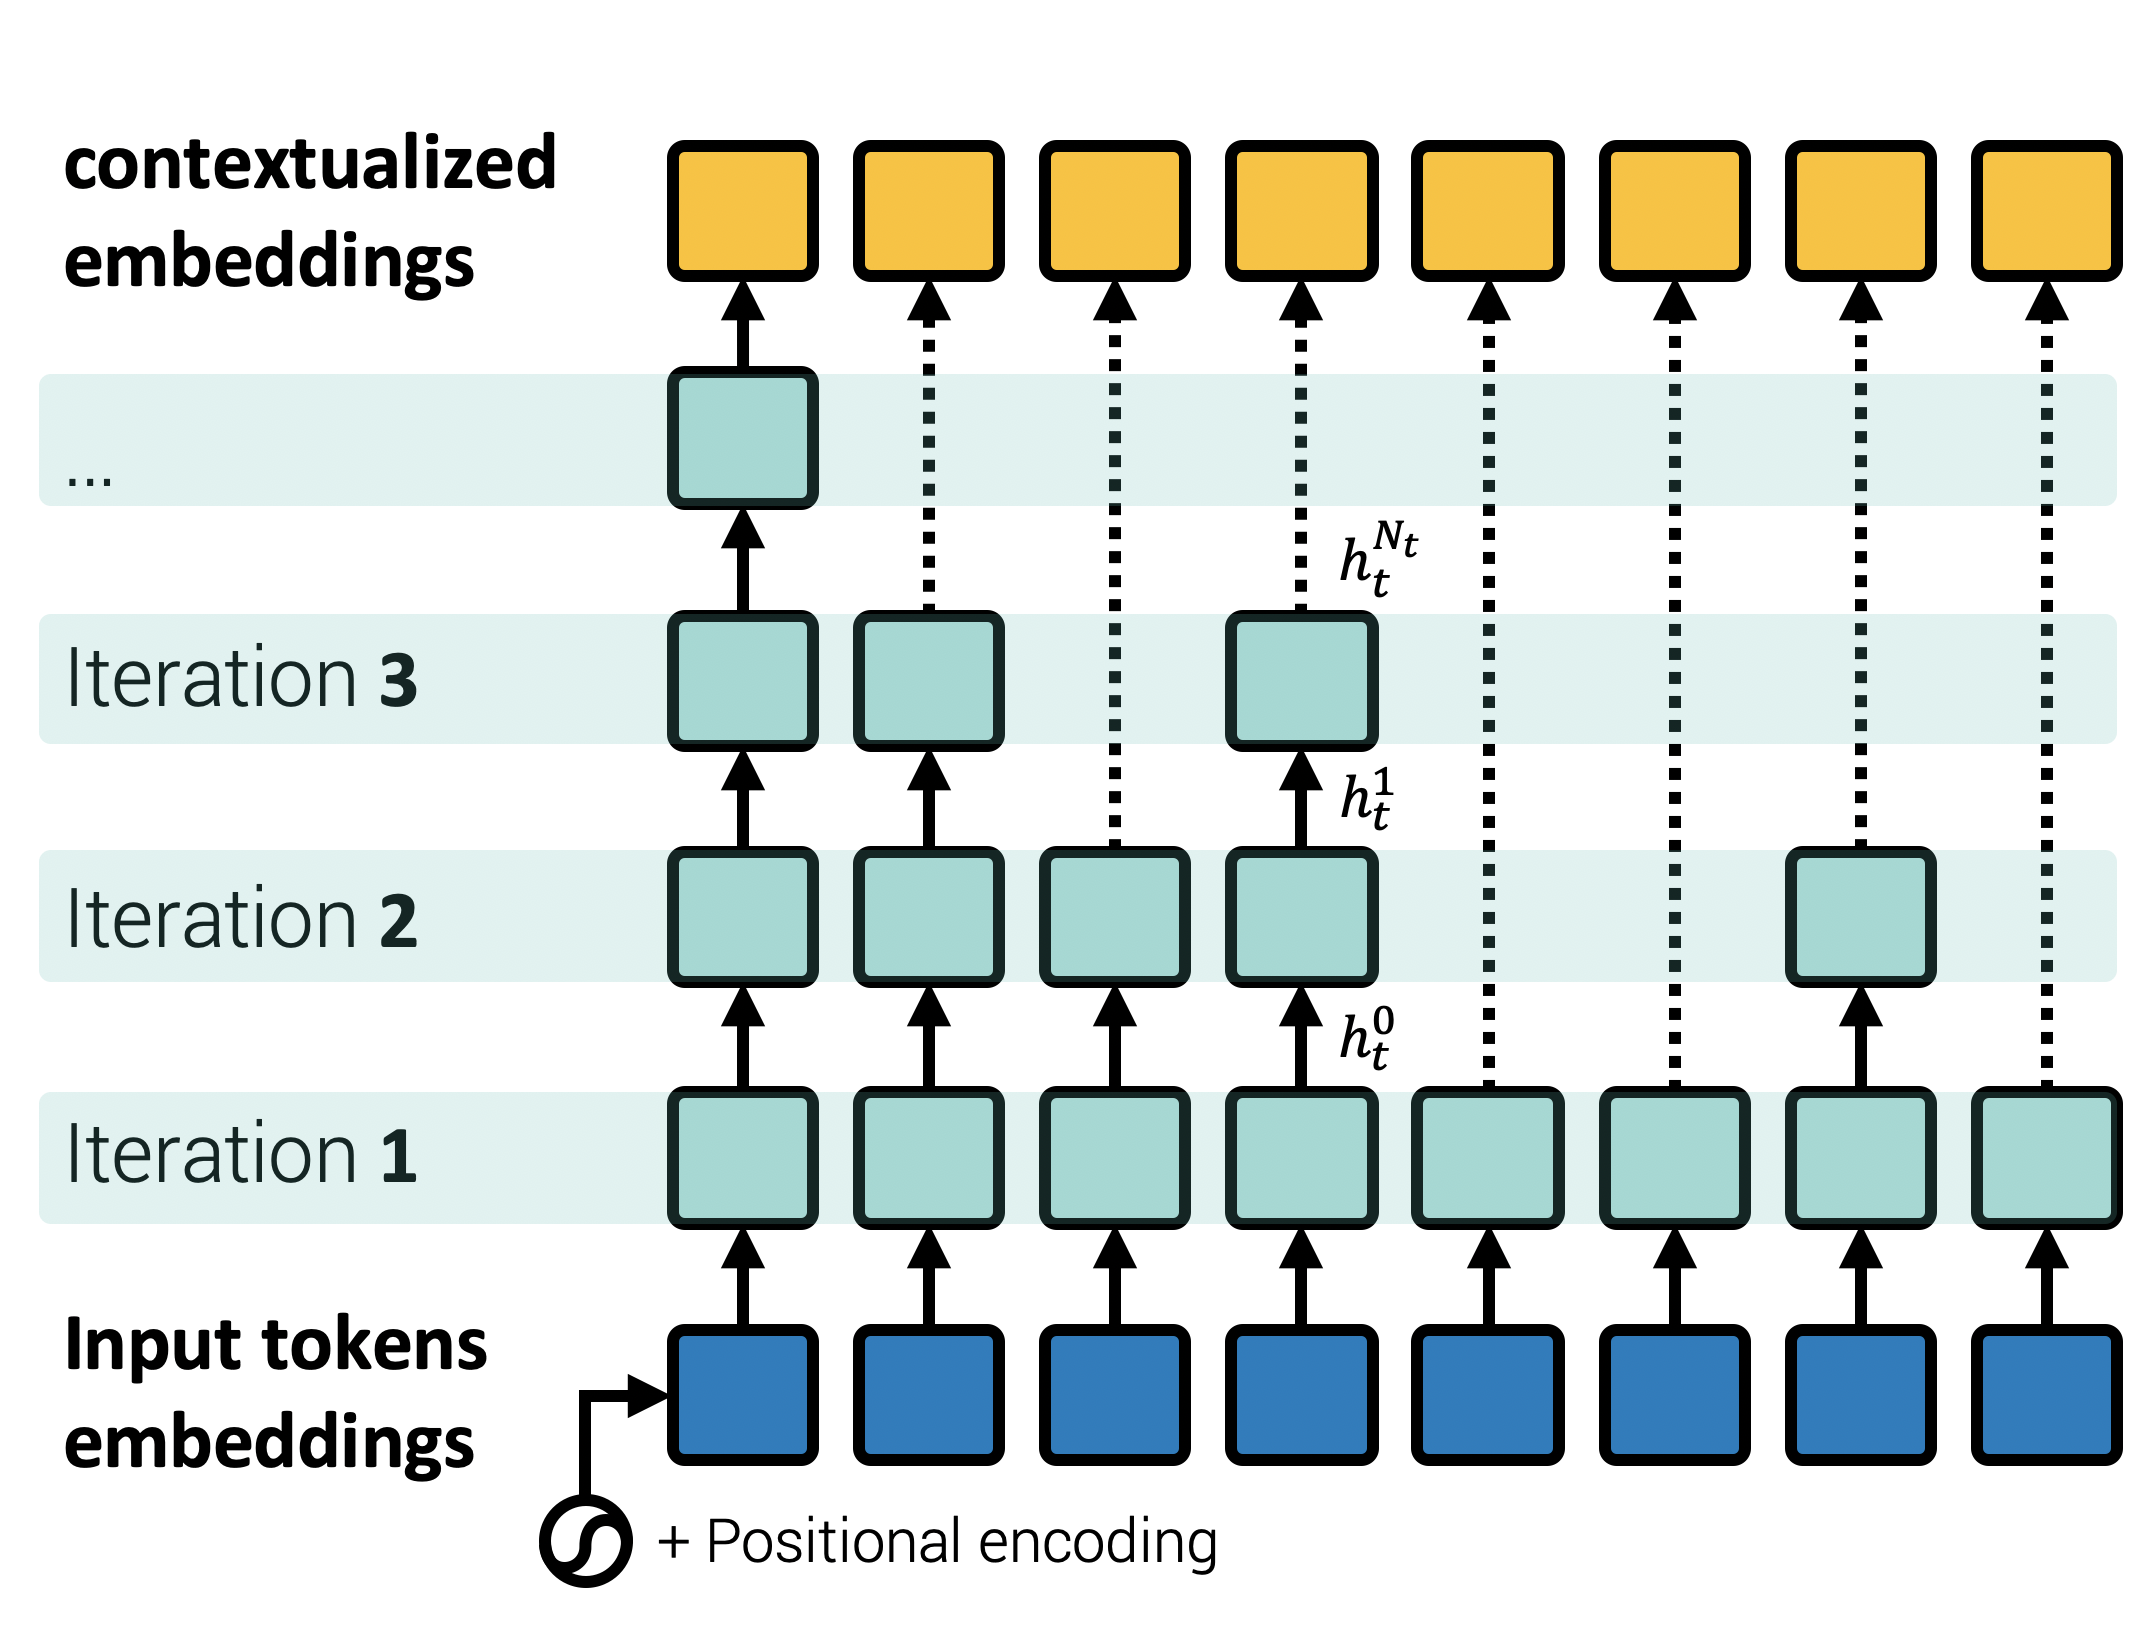
\includegraphics[width=8cm]{images/model-3.png}
\end{center}
\caption{As in \textsc{Albert}  model, tokens are transformed through the iterative application of a transformer encoder layer. Our model's key specificity is the application of the halting mechanism, which dynamically adjusts the number of iterations for each token.
}
\labfig{transformers:model}
\end{figure}

\subsection{Pre-training objective}
\labsec{transformers:pre-training}

During the pre-training phase, we train the model with the sentence order prediction (\textit{sop}) — the task introduced in \textcite{lan_20} that classifies whether segments from the input sequence follow the original order or were swapped — and the masked language model task (\textit{mlm}) \parencite{devlin_19}. We also encourage the network to minimize the number of iterations by directly adding the ponder cost into \textsc{Albert}  pre-training objective. Given a length $T$ input sequence $\textbf{u}$,  \textcite{graves_16} defines the \emph{ponder cost} $\mathcal{P}(\textbf{u})$ as:
\begin{equation}
% \mathcal{P}(\textbf{u}) &= \sum_{t=1}^T N_{t} + R_t^{N_{t}-1} \label{eq:ponder-cost}\\
\mathcal{P}(\textbf{u}) = \sum_{t=1}^T N_{t} + R_t \label{eq:ponder-cost}
\end{equation}

We define the final pre-training loss as the following sum:

\begin{equation}
\hat{\mathcal{L}} = \mathcal{L}_{sop} + \mathcal{L}_{mlm} + \tau \mathcal{P} \label{eq:ponder-loss}
\end{equation}
where $\tau$ is a \emph{time penalty} parameter that weights the relative cost of computation versus error.

\subsection{Datum and infrastructure}
\labsec{transformers:datum}

We follow the protocol from \textsc{Albert} and pre-train the model with \textsc{BookCorpus}~\parencite{zhu_15} and English Wikipedia. We reduce the maximum input length to 128 and the number of training steps to \numprint{112500}\sidenote{As emphasized in \url{https://github.com/google-research/bert}, longer sequences are computationally expensive. To lighten the pre-training process, they advise using 128 sentence length and increasing the length to 512 only for the last 10\% of the training to train the positional embeddings. In this work, we only perform the first 90\% steps as we are not looking for brute force performances.}. We use a lowercase vocabulary of size \numprint{30000} tokenized using SentencePiece. We train all our models on a single TPU v2-8 from Google Colab Pro\sidenote{\url{https://colab.research.google.com/}} and accumulate gradients to preserve a \numprint{4096} batch size. We optimize the parameters using \textsc{Lamb} with a learning rate at 1.76e-3.

\section{Experiments}
\labsec{transformers:experiments}

%We presented in Section~\ref{sec:method} the architecture of our iterative transformer model. 
We now analyze our iterative model properties during pre-training (\refsec{transformers:analysis-pretraining}) and fine-tuning (\refsec{transformers:analysis-downstream}). We start by describing the setup for each of the subtasks.

% \subsection{Experimental setup}
% \label{sub-sec:experimental-setup}

\paragraph{Masked language model (\textit{mlm}) task} We generate masked inputs following \textsc{Albert} $n$-gram masking. We mask 20\% of all WordPiece tokens but do not always replace masked words with the \texttt{[MASK]} token to avoid discrepancy between pre-training and fine-tuning. We effectively replace 80\% of the masked position with \texttt{[MASK]} (\texttt{[MASK/MASK]}), 10\% with a random token (\texttt{[MASK/random]}), and keep the original token for the last 10\% (\texttt{[MASK/original]}).

\paragraph{Next sentence prediction (\textit{sop}) task} We format our inputs as ``\texttt{[CLS]} $x_1$ \texttt{[SEP]} $x_2$ \texttt{[SEP]}''. In 50\% of the case the two segments $x_1$ and $x_2$ are effectively consecutive in the text. In the other 50\%, the segments are swapped. 
% The \textit{sop} task discriminates between the two cases.

\paragraph{Ponder cost} We fix the time penalty factor $\tau$ empirically such that the ponder penalty represents around 10\% of the total loss. To estimate the ponder cost, we discard the remainder as $R \ll N$ for sufficient values of $N$. Given Eq.~\ref{eq:ponder-cost}, the ponder cost then corresponds to the total number of iterations in the sentence, which is given by $l \times T$, with $T$ the number of tokens in the sequence and $l$ the average iterations per token. We observe that \textsc{Albert} base loss converges to around 3.5. We calibrate $\tau$ such that  $\tau\mathcal{P} \approx 0.35 \approx \tau \times l \times T$. We train distinct models, listed in \reftab{transformers:pre-training}, that we calibrate such that their average number of iterations per token $l$ is respectively 3, 6, and 12. We refer to these models as respectively \textit{tiny}, \textit{small} and \textit{base}. 

\subsection{Analysis of the pre-training}
\labsec{transformers:analysis-pretraining}

% \begin{table*}[!htb]
% \small
% \renewcommand{\arraystretch}{1.2}
% \begin{center}
%  \begin{tabular*}{\textwidth}{l@{\extracolsep{\fill}}cccccccc c}
%     \toprule
%  &  MNLI-(m/mm)    & QQP        & QNLI       & SST-2      & CoLA       & STS-B      & MRPC       & RTE        & \textbf{Average} \\
%  & 392k            & 363k       & 108k       & 67k        & 8.5k       & 5.7k       & 3.5k       & 2.5k       & -          \\ 
% % \midrule\multicolumn{10}{c}{\it GLUE Leaderboard} \\\midrule
% % Pre-OpenAI SOTA    & 80.6/80.1       & 66.1       & 82.3       & 93.2       & 35.0       & 81.0       & 86.0       & 61.7       & 74.0       \\
% % BiLSTM+ELMo+Attn   & 76.4/76.1       & 64.8       & 79.8       & 90.4       & 36.0       & 73.3       & 84.9       & 56.8       & 71.0       \\
% % OpenAI GPT         & 82.1/81.4       & 70.3       & 87.4       & 91.3       & 45.4       & 80.0       & 82.3       & 56.0       & 75.1       \\
% % \textsc{Bert}-base          & 84.6/83.4       & 71.2       & 90.5       & 93.5       & 52.1       & 85.8       & 88.9       & 66.4       & 79.6       \\
% % \textsc{Albert}-base          & 84.6/83.4       & 71.2       & 90.5       & 93.5       & 52.1       & 85.8       & 88.9       & 66.4       & 79.6       \\
% \midrule\multicolumn{10}{c}{\it GLUE Leaderboard Reproductions} \\\midrule
% \textsc{Bert}-base          & 82.3/81.4       & 70.8       & 89.3       & 92.0       & 38.8       & 84.0       & 87.1       & 65.4       & 76.9       \\
% \textsc{Albert}-base          & ---/---       & ---       & ---       & ---       & ---       & ---       & ---       & ---       & ---       \\
% \midrule\multicolumn{10}{c}{\it Our Models} \\\midrule
% \textsc{Albert}-tiny + Adapt. Depth          & 77.0/76.8   & 67.8    & 86.4       & 87.6       & 27.5       & 81.8         &  84.7       & 62.0       & 72.6       \\
% \textsc{Albert}-small + Adapt. Depth          &   79.5/78.5     & 67.8       & 88.3       & 88.6       & 33.8       & 82.7       & 85.2      & 61.9       & 74.2       \\
% \textsc{Albert}-base + Adapt. Depth          & 79.9/79.2       & 68.5       & 89.0       & 87.8       & 36.7       & 84.2       & 86.5       & 63.0       & 75.2       \\
%     \bottomrule
%    \end{tabular*}
%    \caption{GLUE Test results}
%    \label{tab:glue_official}
% \end{center}
% \end{table*}

\paragraph{Analysis of the iterations} We pre-train models with various configurations and observe the model mechanisms during the pre-training in \reftab{transformers:pre-training}. 

\begin{table}[!htb]
% \footnotesize
\small
% \begin{minipage}{\textwidth}
\centering {
\begin{tabularx}{\textwidth}{l@{\extracolsep{\fill}}c c c c@{}}
\toprule
Models & \textit{tiny} & \textit{small} & \textit{base}\\
\midrule
% $\tau$ & 1e-3 & 5e-4 & 2.5e-4\\
% Max iterations & 6 & 12 & 24\\
% mlm (Acc.) & 55.4 & 57.1 & 57.4\\
% sop (Acc.) & 80.9 & 83.9 & 84.3\\
% \midrule
% All tokens & 3.8 & 6.9 & 9.8\\
% % \textbf{[MASK]} & 5.8 & 10.9 & 16\\
% All unmasked tokens & 3.6 & 6.4 & 9.2\\\relax
% \texttt[MASK/MASK]} & 5.8 & 10.9 & 16.0\\\relax
% \texttt[MASK/random]} & 5.8 & 10.9 & 16.0\\\relax
% \texttt[MASK/original]} & 4.0 & 7.4 & 10.5\\\relax
% \texttt[CLS]} & 5.7 & 10.4 & 18.9\\\relax
% \texttt[SEP]} & 2.3 & 5.7 & 8.1\\
$\tau$ & 1e-3 & 5e-4 & 2.5e-4\\
Max iterations & 6 & 12 & 24\\
mlm (Acc.) & 55.4 & 57.1 & 57.4\\
sop (Acc.) & 80.9 & 83.9 & 84.3\\
\midrule
All tokens & 3.8 & 7.1 & 10.0\\
All unmasked tokens & 3.5 & 6.5 & 9.2\\\relax
\texttt{[MASK/MASK]} & 5.8 & 10.9 & 16.0\\\relax
\texttt{[MASK/random]} & 5.8 & 10.9 & 16.0\\\relax
\texttt{[MASK/original]} & 4.0 & 7.4 & 10.5\\\relax
\texttt{[CLS]} & 6.0 & 12.0 & 22.5\\\relax
\texttt{[SEP]} & 2.5 & 7.6 & 8.4\\
\bottomrule
\end{tabularx}}
\caption{Average number of iterations given token types during the pre-training. For each model, we report a mean number of iterations on our development set, at the end of the pre-training. 
%We make the distinction between each configuration.
}
\labtab{transformers:pre-training}
\end{table}

% Regarding the special tokens, we confirm results advanced by the analysis of \textsc{Bert}  attention patterns \parencite{clark_19}. 
We observe that the \texttt{[CLS]} token receives far more iterations than other tokens. This observation is in line with \textcite{clark_19} who analyze \textsc{Bert}  attention and report systematic and broad attention to special tokens. We interpret that the \texttt{[CLS]} token is used as input for the \textit{sop} task and aggregates a representation for the entire input. On the contrary, \texttt{[SEP]} token benefits from usually few iterations. Again, this backs up the observation emerging from the analysis of attention that interprets \texttt{[SEP]} as a no-op operation for attention heads \parencite{clark_19}.

% We interpret that the \texttt{[CLS]} token is used for the \textit{sop} objective, which depends on every other token in the sentence. The \texttt{[CLS]} token acts as an artificial root of the sentence and needs other tokens to converge before its.   

We also observe an interesting behavior from the \texttt{[MASK]} which also benefits from more iterations than average tokens. As for the \texttt{[CLS]} token, we interpret that these tokens are crucial for the \textit{mlm} task. Looking further, we observe that \texttt{[MASK/random]} and \texttt{[MASK/MASK]} number of iterations is greater than \texttt{[MASK/original]}. In this case, although all tokens are targeted in the \textit{mlm} task, \texttt{[MASK/random]} and \texttt{[MASK/MASK]} are  obviously more difficult to identify\sidenote{During inference, the model cannot make the distinction between \texttt{[MASK/original]} and unmasked tokens. However, we observe in \reftab{transformers:pre-training} that the two token types have a distinct mean number of iterations. We believe this is due to the distribution of the \texttt{[MASK]} tokens. Indeed, we follow the procedure from \textsc{Albert}  and use \textit{n-gram} masking. Therefore, \texttt{[MASK/original]} tokens tend to appear in the context of \texttt{[MASK]} tokens. This specific context increases the mean number of iterations.}.
%more explicit and less difficult to identify than

The model seems to have an intuitive mechanism and distributes iterations for tokens that are either crucial for the pre-training task or present a certain difficulty level. This also appears in line with \textit{early-exit} mechanisms cited in \refsec{transformers:dynamic-depth}, that adapts the number of iterations, for the whole example, to better scale to each sample level of difficulty.

% We observe that mask tokens benefit from more iterations. We observe a discrepancy between these categories. In particular, when the mask token is unchanged, the number of iterations stands between unmask tokens and other mask tokens. We interpret that tokens are directly driven by the loss benefit from more iterations and that, as expected, ambiguous tokens such as \texttt{[MASK]} require more iterations.

\paragraph{Natural Fixed point} We now analyze \textit{how} the token's hidden states evolve during our model iterative transformations. At each iteration $n$, the self-attentive mechanism \parencite{vaswani_17} computes the updated state $n+1$ as a weighted sum of the current states. This introduces a cyclic dependency as every token depends on each other during the iterative process. As convergence within a loopy structure is not guaranteed, we encourage the model to converge towards a fixed point \parencite{bai_19}.

\begin{figure}[!htb]
\begin{center}
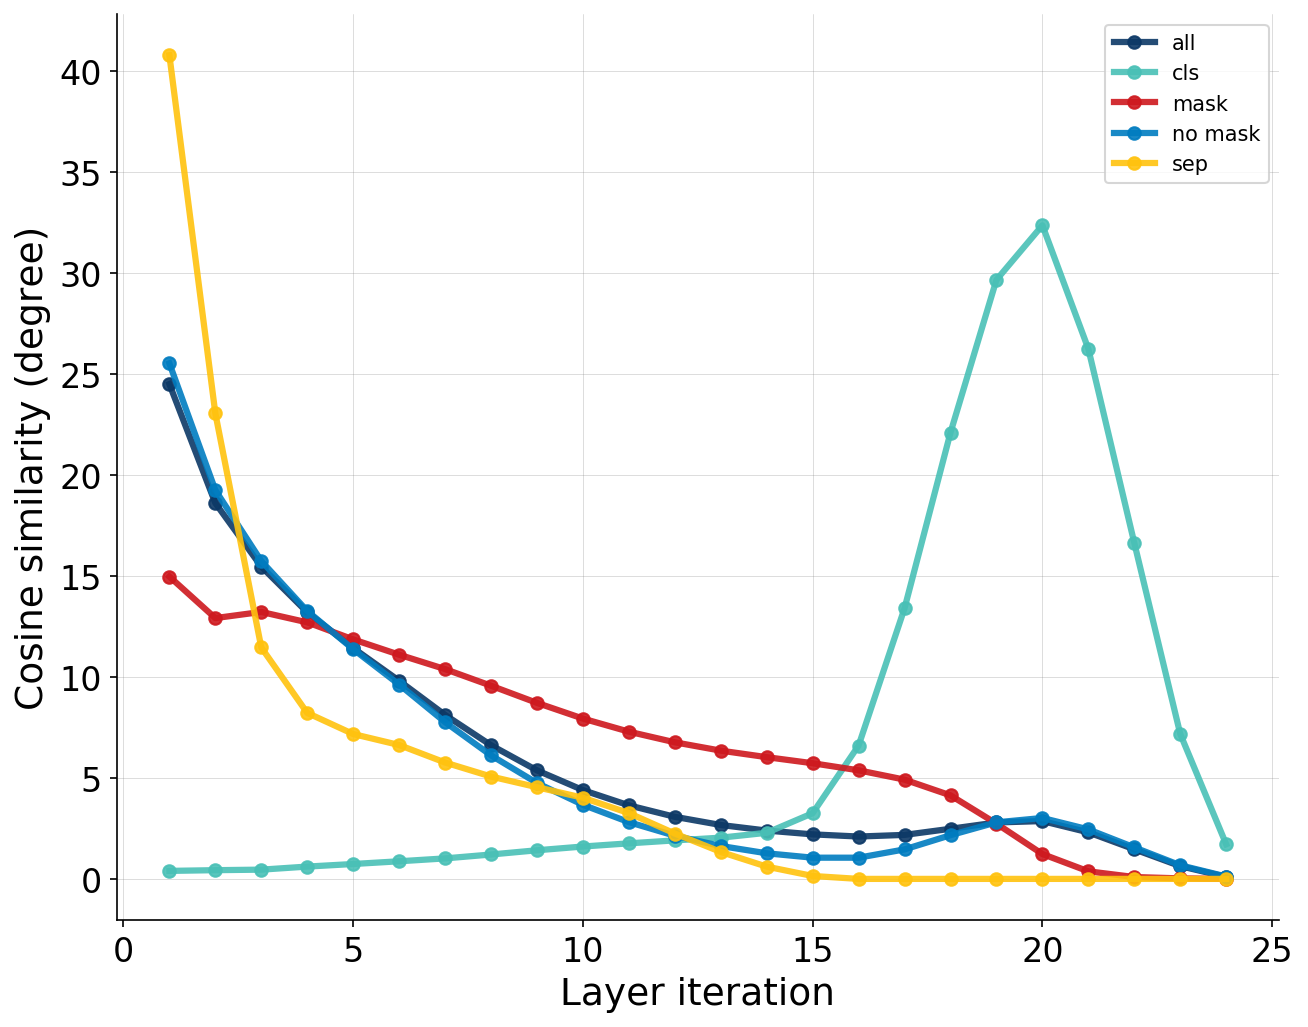
\includegraphics[width=8cm]{images/cosine-base-v3 (1).png}
\end{center}
\caption{Evolution of the cosine similarity between hidden states $h^n_t$ and $h^{n+1}_t$ from two consecutive iterations. We use our \textit{base} model and measure iterations on our development set at the end of the pre-training.}
\labfig{fixed-point}
\end{figure}

We obtain this property "for free" thanks to our architecture specificity. Indeed at each iteration, the hidden state is computed as a convex combination of the previous $n$ and current $n+1$ hidden state. The combination is controlled by $\lambda^n_t$  (Eq.~\ref{eq:halting-3}). If $\lambda^n_t$ is closed to $0$, then $h^n_t \approx h^{n+1}_t$ and by definition (Eq.~\ref{eq:halting-22}, \ref{eq:halting-r}) $\lambda^n_t$ will eventually be set to $0$ at a certain iteration.

% we encourage the model to reach a fixed point \parencite{bai_19}. Indeed, transformers induce a dependency between every token in the sentence as the self-attentive mechanism \parencite{vaswani_17} computes each state as a weighted sum from each other. This introduces a cyclic dependency between each token. Convergence within a loopy structure is known to be uncertain. We encourage the model to reach a fixed point, to facilitate the convergence process. 

% By design, we encourage the model to converge toward a fixed point. This property may be used as a sole training objective \parencite{bai_19} while we obtain this property "for free" thanks to the specificity of our architecture. 


\reffig{fixed-point} represents the evolution of the mean cosine similarity between two hidden states from two consecutive iterations $h^n_t$ and $h^{n+1}_t$. The network indeed reaches a fixed point for every token. The \texttt{[SEP]} and tokens that are not masked converge quicker than \texttt{[MASK]} tokens. Finally, the \texttt{[CLS]} token oscillates during intermediate iterations before reaching an equilibrium.
% \sidenote{We present the Figures for other model configurations in Appendix~\ref{appendix:natural-fixed-point}}.

\subsection{Application to downstream tasks}
\labsec{transformers:analysis-downstream}

During the pre-training phase, the model focuses on tokens either crucial for the pre-training task or that present a certain level of difficulty. Now, we study our model behavior during the fine-tuning on downstream syntactic or semantic tasks.


\paragraph{Control test} To verify that our setup has reasonable performance, we evaluate it on the GLUE benchmark \parencite{wang_19}.
% \sidenote{We provide experimental details in Appendix~\ref{appendix:glue}}. 
Results from \reftab{glue-official} are scored by the evaluation server\sidenote{\url{https://gluebenchmark.com/leaderboard}}. As in \textcite{devlin_19}, we discard results for the WNLI task\sidenote{See point (12) from \url{https://gluebenchmark.com/faq}.}. For each task, we fine-tune the model on the train set and select the hyperparameters on the dev set using a grid search. We tune the learning rate between 5e-5, 3e-5, and 2e-5; batch size between 16 and 32, and epochs between 2, 3, or 4. To better compare our setup, we pre-train \textsc{Bert} and \textsc{Albert} model using our configuration, infrastructure, and datum.

\begin{table}[!htb]
\small
%\renewcommand{\arraystretch}{1.2}
\centering {
\begin{tabularx}{\textwidth}{l@{\extracolsep{\fill}} Y Y@{}}
\toprule
& \textbf{Avg. Glue score} \\
\midrule
\textsc{Bert}-base   & 76.9       \\
\textsc{Albert}-base   & 75.6       \\
\midrule
\textsc{Albert}-base + Adapt. Depth  & 75.2       \\
\textsc{Albert}-small + Adapt. Depth     & 74.2       \\
\textsc{Albert}-tiny + Adapt. Depth       & 72.6       \\
\bottomrule
\end{tabularx}}
\caption{GLUE Test results, scored by the evaluation server but without the WNLI task. To facilitate the comparison, we reproduce \textsc{Bert} and \textsc{Albert}, with our pre-training dataset, infrastructure and configuration detailed in \refsec{transformers:pre-training}.}
\labtab{glue-official}
\end{table}

We present results on the test set in \reftab{glue-official}. As expected, the average score decreases with the number of iterations. Indeed, we limit the number of computation operations performed by our model. Moreover, we build our model on top of \textsc{Albert}, which share parameters across layers, thus reducing the number of parameters compared with the original \textsc{Bert}  architecture. However, despite these additional constraints, results stay in a reasonable range. In particular, \textsc{Albert}-base with adaptative depth is very close to the version with a fixed depth. 
%Although, as detailed in Table~\ref{table:pre-training}, tokens perform in average only 10 iterations compared to 12 for \textsc{Albert}-base.

%\sidenotetext{See (10) in \url{https://gluebenchmark.com/faq}.}
% . scored by the evaluation server ({\small \url{https://gluebenchmark.com/leaderboard}}). The number below each task denotes the number of training examples. The ``Average'' column is slightly different than the official GLUE score. since we exclude the problematic WNLI set.\sidenote{See question 10 in \url{https://gluebenchmark.com/faq}.} 
   %OpenAI GPT = (L=12. H=768. A=12); \textsc{Bert} base = (L=12. H=768. A=12); \textsc{Bert} large = (L=24. H=1024. A=16).  BERT and OpenAI GPT are single-model. single task. F1 scores are reported for QQP and MRPC. Spearman correlations are reported for STS-B. and accuracy scores are reported for the other tasks. We exclude entries that use BERT as one of their components.


\paragraph{Probing tasks} \textcite{conneau_18} introduce probing tasks, which assess whether a model encodes elementary linguistic properties. Such tasks are detailed in \refsec{survey:probing} We consider semantic and syntactic tasks that do not introduce random replacements. In particular, a task that predicts the sequence of top constituents immediately below the sentence node (TopConst), a task that predicts the tense of the main-clause verb (Tense), and two tasks that predict the subject (resp. direct object) number in the main clause (SubjNum, resp. ObjNum). We provide examples for each of these tasks in \reftab{senteval:probing-examples}.

\begin{table*}[!htb]
\footnotesize
\centering {
\begin{tabularx}{16cm}{@{}X c@{}}
\toprule
\textbf{Sentence} & \textbf{Label} \\
\midrule\midrule
\multicolumn{2}{c}{\textit{Tense}}\\\midrule
The smell churned my stomach even faster . & PAST\\
I lean against the post and watch her set up . & PRES\\
\midrule
\multicolumn{2}{c}{\textit{Subj Num}}\\\midrule
The crows circled above me . & NNS\\
" I imagine it 's nothing good , but speak , " the colonel said . & NN\\
\midrule
\multicolumn{2}{c}{\textit{Obj Num}}\\\midrule
I saw the ramp leading back toward the surface . & NN\\
I could feel their stares like hot rays penetrating into me . & NNS\\
\midrule
\multicolumn{2}{c}{\textit{Top Const}}\\\midrule
They obviously protect him from anything he won 't like . & S\_NP\_VP\_.\\
Did it belong to the owner of the house ? & VBD\_NP\_VP\_.\\ 
\bottomrule
\end{tabularx}}
\caption{\labtab{senteval:probing-examples} Examples from the tasks of the probing tasks \parencite{baroni_18} of the SentEval benchmark that we will use in our experiments. The top constituent task (\textbf{TopConst}), aims at predicting the top constituent immediately below the sentence root node. The \textbf{Tense} task aims at predicting the tense of the main clause verb. The subject and object number (respectively \textbf{SubjNum} and \textbf{ObjNum}) tasks focus on the number of respectively the subject and object of the main clause. All sentences are extracted from the Toronto Book Corpus \parencite{zhu_15}. The part-of-speech, constituency and dependency parsing information are provided with the Stanford Parser (2017-06-09 version), using the pre-trained PCFG model \parencite{klein_2003}. The top constituent task (\textbf{TopConst}) classifies sentences on the basis of their sequences of top constituents immediately below the sentence node. There are 19 classes for the most frequent top constructions, and one for all other constructions.}%
\end{table*}
% \bcomment{for SUbjNum,ObjNum,Top Const please specify that the labels come from the Penn Treebank. I do not understand the labels for top const }{}


% model small warm up 3000 5e-5
% \begin{table}[!htb]
% \small
% % \begin{minipage}{\textwidth}
% \centering {
% \begin{tabularx}{\textwidth}{l@{\extracolsep{\fill}}Y Y Y Y Y@{}}
% \toprule
%   & Tense & Subj Num & Obj Num & Top Const\\
% \midrule
% punct (121k)      & 3.2 & 2.6 & 3.4 & 3.8\\
% prep (101k)      & 3.0 & 2.5 & 3.1 & 3.3\\
% pobj (98k)      & 3.0 & 2.6 & 3.1 & 3.2\\
% det (86k)      & 2.9 & 2.4 & 3.0 & 3.4\\
% nn (81k)     & 3.2 & \textbf{3.0} & 3.3 & 3.6\\
% nsubj (80k)      & \textbf{3.4} & \textbf{3.2} & \textbf{3.3} & \textbf{4.1}\\
% amod (66k)     & 3.0 & 2.6 & 3.2 & 3.4 \\
% dobj (49k)     & 3.1 & 2.7 & \textbf{3.5} & 3.4 \\
% root (44k)     & \textbf{3.6} & \textbf{3.1} & \textbf{3.7} & \textbf{4.4} \\
% advmod (37k)     & 3.1 & 2.5 & 3.2 & 3.7 \\
% \midrule
% avg.      & 3.2 & 2.8 & 3.4 & 3.6 \\
% % std.      & 0.2 & 0.3 & 0.2 & 0.5 \\
% test Acc.      & 89.8 & 93.0 & 94.7 & 90.8 \\
% baseline Acc.      & 90.6 & 93.3 & 96.1 & 91.3 \\

% \bottomrule
% \end{tabularx}}
% \caption{Distribution of the iteration across token dependency types. We fine-tune our \textit{small} model on each probing task. We the perform inference on the Penn Tree Bank dataset and report the number of iterations given token dependency types. The number in parentheses denotes the number of dependency tags. We only display the top 10 most frequent tags. We indicate in \textbf{bold} tags  for  which the iteration is above avg + std. We include a baseline accuracy which we obtain with the \textsc{Albert} -base version without an adaptative depth mechanism and therefore 12 iterations performed for each token.}
% \label{table:probing}
% \end{table}

% model base warm up 3000 5e-5
% \begin{table}[!htb]
% \small
% % \begin{minipage}{\textwidth}
% \centering {
% \begin{tabularx}{\textwidth}{l@{\extracolsep{\fill}}Y Y Y Y Y@{}}
% \toprule
%   & Tense & Subj Num & Obj Num & Top Const\\
% \midrule
% punct (121k)      & 7.2 & 6.6 & 7.1 & \textbf{7.0}\\
% prep (101k)      & 6.6 & 6.0 & 6.9 & 6.1\\
% pobj (98k)      & 6.7 & 6.0 & 7.0 & 5.9\\
% det (86k)      & 6.5 & 5.9 & 6.6 & 6.2\\
% nn (81k)     & 7.2 & 6.8 & 7.4 & 6.5\\
% nsubj (80k)      & \textbf{7.6} & \textbf{7.5} & \textbf{7.6} & \textbf{7.6}\\
% amod (66k)     & 6.6 & 6.1 & 6.9 & 6.0 \\
% dobj (49k)     & 6.9 & 6.3 & \textbf{7.5} & 6.0 \\
% root (44k)     & \textbf{8.1} & \textbf{7.7} & \textbf{7.9} & \textbf{7.7} \\
% advmod (37k)     & 6.8 & 6.3 & 6.9 & \textbf{6.9} \\
% \midrule
% avg.      & 7.5 & 6.9 & 7.7 & 7.2 \\
% % std.      & 0.2 & 0.3 & 0.2 & 0.5 \\
% test Acc.      & 90.4 & 94.2 & 95.9 & 91.1 \\
% baseline Acc.      & 90.6 & 93.3 & 96.1 & 91.3 \\

% \bottomrule
% \end{tabularx}}
% \caption{Distribution of the iteration across token dependency types. We fine-tune our \textit{small} model on each probing task. We the perform inference on the Penn Tree Bank dataset and report the number of iterations given token dependency types. The number in parentheses denotes the number of dependency tags. We only display the top 10 most frequent tags. We indicate in \textbf{bold} tags  for  which the iteration is above avg + std. We include a baseline accuracy which we obtain with the \textsc{Albert} -base version without an adaptative depth mechanism and therefore 12 iterations performed for each token.}
% \label{table:probing}
% \end{table}

In our setup, we fine-tune the model on the task train set and select the hyperparameters on the dev set using a grid search. We use a 5e-5 learning rate and fine-tune the epochs between 1 to 5; we use a 32 batch size.
%we fine-tune the model on the task train set. We select the best number of training steps on the dev set. 
Finally, we %perform inference and 
compare in Table~\reftab{table:probing} the number of iterations performed for each token 
% measure the number of iterations performed for each token 
on the Penn Tree Bank \parencite{marcus_94} converted to Stanford dependencies\sidenote{Since we use sentence piece vocabulary, we assign to each piece the dependency tag from the whole token.}.
%\sidenote{We present the Tables for other model configurations in Appendix~\ref{appendix:probing}}.
% We compare in Table~\ref{table:probing} the number of iterations performed for each token 

We provide an accuracy baseline, obtained with the same setup but using \textsc{Albert}  without the dynamic halting mechanism. As in the previous experiment, we observe that for these tasks, our model achieves competitive performances despite using less computational operations.

Although all tasks achieve significant and comparable accuracies, they all require a distinct global mean of iterations. The Tense task, which can be solved from the verb only, is completed in only 5.4 iterations, while the TopConst task, which requires inferring some sentence structure, is performed in \textbf{7.2} iterations. This suggests the model can adapt itself to the complexity of the task and globally spare unnecessary iterations. 

Looking at the token level, as during the pre-training (\refsec{transformers:analysis-pretraining}), the iterations are unevenly distributed across tokens. The model seems to iterate more on crucial tokens for the task. For SubjNum, the subj tokens achieve the maximum number of iterations, while for the ObjNum task, the obj and root token iterates more. Similarly, all tasks present many iterations on the main verb (root) that is crucial for each prediction.

% model base warm up 200 5e-5
\begin{table}[!htb]
\small
% \begin{minipage}{\textwidth}
\centering {
\begin{tabularx}{\textwidth}{l@{\extracolsep{\fill}}Y Y Y Y Y@{}}
\toprule
  & Tense & Subj Num & Obj Num & Top Const\\
\midrule
punct (121k)      & 5.0 & 4.8 & 5.2 & 6.7\\
prep (101k)      & 4.6 & 4.6 & 5.4 & 6.2\\
pobj (98k)      & 4.5 & 4.6 & 5.4 & 5.8\\
det (86k)      & 4.5 & 4.6 & 5.1 & 6.1\\
nn (81k)     & 5.1 & 5.4 & \textbf{5.8} & 6.7\\
nsubj (80k)      & \textbf{5.3} & \textbf{6.1} & \textbf{5.9} & \textbf{7.5}\\
amod (66k)     & 4.6 & 4.9 & 5.5 & 6.1 \\
dobj (49k)     & 4.8 & 5.0 & \textbf{5.9} & 6.1 \\
root (44k)     & \textbf{5.9} & \textbf{6.1} & \textbf{6.2} & \textbf{7.9} \\
advmod (37k)     & 4.8 & 4.8 & 5.3 & 6.8 \\
\midrule
avg.      & 5.4 & 5.4 & 5.8 & 7.2 \\
% std.      & 0.2 & 0.3 & 0.2 & 0.5 \\
test Acc.      & 87.5 & 93.9 & 96.1 & 91.2 \\
baseline Acc.      & 87.3 & 94.0 & 96.0 & 91.9 \\
\bottomrule
\end{tabularx}}
\caption{Distribution of the iterations across token dependency types. We fine-tune our \textit{base} model on each probing task. We then perform inference on the Penn Tree Bank dataset and report the number of iterations given token dependency types. In parentheses, we indicate the number of occurrences for each dependency tag. We only display the top 10 most frequent tags. We indicate in \textbf{bold} tags for which the number of iterations is above avg + std. We include a baseline accuracy which we obtain with the \textsc{Albert}-base version without an adaptative depth mechanism, and therefore 12 iterations were performed for each token.}
\labtab{table:probing}
\end{table}

\section{Conclusion and future work}
% We propose a transformer pre-trained model that adapts the number of layer iterations performed on each token. We assume that language have a recursive structure where tokens, such as verbs, induce more dependence with other tokens than determinant or adverbs for example. We hypothesize that computing contextualized representation for a given token requires first computing the representation for its dependants. Therefore, we expect low dependency tokens to quickly converge in the early layer, while highly dependent, complex, or ambiguous tokens would converge in later layers. Exiting the process early for low dependency or explicit tokens may spare some computations and avoid interference with the global convergence process.

% To this end, 
We investigated the role of the layers in deep transformers. We designed an original model that progressively transforms each token through a dynamic number of iterations. We analyzed the distribution of these iterations during pre-training and confirmed the results obtained by analyzing the distribution of attention across \textsc{Bert} layers, particularly the specific behavior played by special tokens. Moreover, we observed that key tokens for the prediction task benefit from more iterations. We confirmed this observation during fine-tuning, where the tokens with a large number of iterations are also suspected to be key for achieving the task.

Our experiments provide a new interpretation path for the role of layers in deep transformer models. Rather than extracting some specific features at each stage, layers could be interpreted as iterations from a convergent process. We hope that this can help to better understand the convergence mechanisms for transformers models, reduce the computational footprint or provide new regularization methods.
